\chapter{Electromagnetic Fields}
The electromagnetic fields are a collection of closely linked fields.
These fields govern the electric and magnetic interactions of charged
particles and domains. These fields can be seen in table \ref{tab:fields}

\begin{table}[h!]
    \begin{center}
        \begin{tabular}{c c c}
            Field    & SI unit                & Description              \\
            \hline
            $\vb{H}$ & $1\, \text{Am}^{-1} $  & Magnetic Field           \\
            $\vb{E}$ & $1\, \text{Vm}^{-1} $  & Electric Field           \\
            $\vb{B}$ & $1\, \text{Vsm}^{-2} $ & Magnetic Flux Density    \\
            $\vb{D}$ & $1\, \text{Asm}^{-2} $ & Electric Flux Density    \\
            $\vb{J}$ & $1\, \text{Am}^{-2} $  & Electric Current Density \\
            $\rho$   & $1\, \text{Asm}^{-3} $ & Electric Charge Density
        \end{tabular}
        \caption{Electromagnetic Field Quantities}
        \label{tab:fields}
    \end{center}
\end{table}
These fields are described by Maxwells Equations.
In differential form for the stationary case, these are as follows:

\begin{align}
    \nabla \times \vb{H} & = \vb{J} + \frac{\partial}{\partial t}\vb{D}
    \label{eq:maxwell1}                                                 \\
    \nabla \times \vb{E} & = -\frac{\partial}{\partial t}\vb{B}
    \label{eq:maxwell2}                                                 \\
    \nabla \cdot \vb{B}  & = \vb{0}
    \label{eq:maxwell3}                                                 \\
    \nabla \cdot \vb{D}  & = \rho
    \label{eq:maxwell4}
\end{align}
Since we're dealing with measurement of magnetic fields in this thesis,
equations \ref{eq:maxwell1} and \ref{eq:maxwell3} will naturally be of
the most interest. In simple cases, the $\vb{H}, \vb{D}, \vb{E}$ and
$\vb{B}$ field obey the relations
\begin{align}
    \vb{B} & = \mu \vb{H}
    \label{eq:BHmap}           \\
    \vb{D} & = \epsilon \vb{E}
\end{align}
where $\mu$ is the \emph{magnetic permeability} and $\epsilon$ is the
\emph{electric permittivity} in the domain of interest.
Formally, simple cases are where the fields are located in a medium that is
linear, homogenous across its domain, invariant depending on direction, and
stationary. Since the magnetic measurements are made inside the empty aperture
of the magnet, the domain is only made up of air. Thus, equation \ref{eq:BHmap}
holds, and the magnetic permeability is the one of free space, that is
$\mu = \mu_0 = 4\pi \times 10^{-7} Hm^{-1}$. \cite[Ch.4.1-4.4]{russenschuck_field_2011}


\subsection{Magnetic Flux and Induction}
Magnetic flux $\Phi$ is the surface integral of the $\vb{B}$ field
along the normal vector to the surface.
Mathematically, it is defined as:
\begin{equation}
    \Phi(\area) = \iint\limits_{\area} \vb{B} \cdot \nvec\, d\area
\end{equation}
where $\area$ is the surface, and $\nvec$ is the normal vector to the surface.
We then have the following governing laws of electromagnetism for objects at rest:
\begin{align}
    U(\partial\area)      & = -\frac{d}{dt}\Phi(\area)
    \label{eq:faraday}                                 \\
    \Phi(\partial\Volume) & = 0
    \label{eq:fluxcons}
\end{align}

\begin{figure}
    \centering
    \begin{subfigure}[b]{0.4\textwidth}
        \centering
        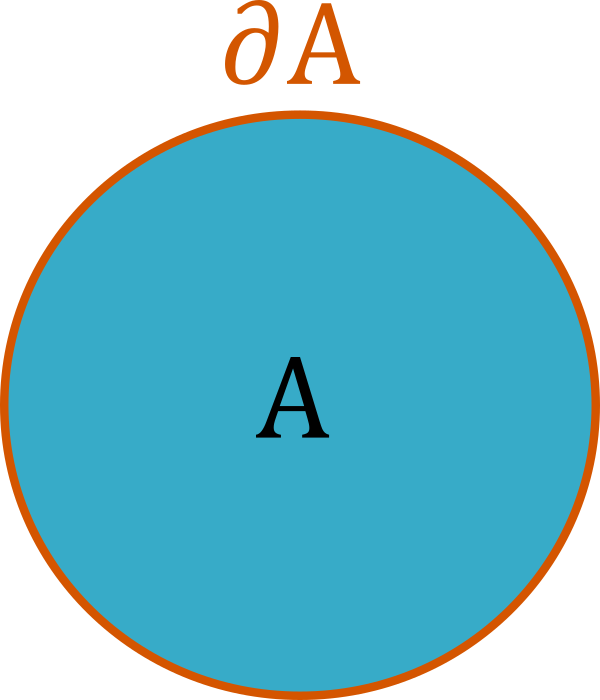
\includegraphics[height=125pt]{figs/partialA}
        \caption{An area $\area$ and its boundary $\partial \area$. }
        \label{fig:partialA}
    \end{subfigure}
    \hfill
    \begin{subfigure}[b]{0.4\textwidth}
        \centering
        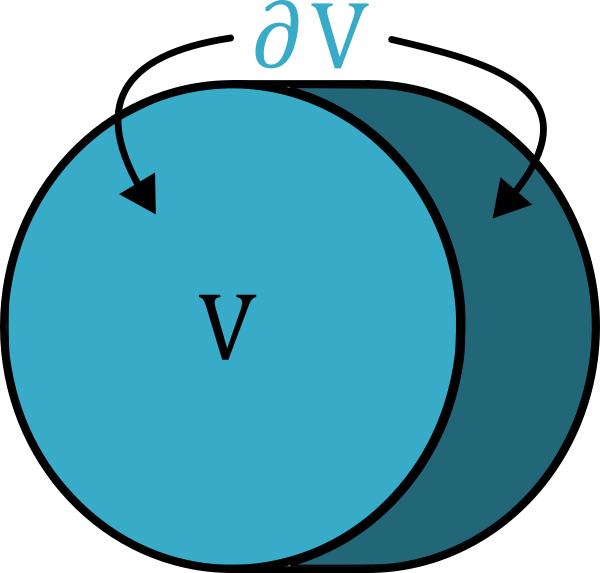
\includegraphics[height=125pt]{figs/partialV}
        \caption{A volume $\Volume$ and its surface boundary $\partial \Volume$.}
        \label{fig:partialV}
    \end{subfigure}
    \caption{}
\end{figure}
Equation \ref{eq:faraday}, also called Faradays law, describes the voltage\
$U$ induced in a length of wire $\partial\area$, enclosing an area
$\area$, when the magnetic flux $\Phi$ is changing with respect to time.
The signs of $U$ and $\Phi$ obey the right hand rule as indicated
in figure \ref{fig:partialA}.

Equation \ref{eq:fluxcons} states that the total amount of flux flowing
through the boundary $\partial\Volume$ of a volume
$\Volume$ must equal zero.\cite[Ch.4.1.1]{russenschuck_field_2011}

\section{Series decompositions of the magnetic field}
\label{sec:series_decompositions}
The magnetic field can be calculated in some different ways, for instance
directly from Maxwells equations or using Biot-Savarts law:
\begin{equation}
    \vb{B}(\vb{r}) = \frac{\mu_0}{4\pi}\int\limits_\Volume
    \frac{\vb{J}(\vb{r'})\times (\vb{r} - \vb{r'})}
    {|\vb{r} - \vb{r'}|^3} d\Volume
    \label{eq:Biot_Savart}
\end{equation}
where $\vb{B}(\vb{r})$ is the $\vb{B}$ field at coordinate $\vb{r}$ and
$\vb{J}(\vb{r'})$ is the current distribution at coordinate $\vb{r'}$.
\cite[Ch.5.4]{russenschuck_field_2011}
Except for very simple geometries, the magnetic field is rarely
expressible using elementary functions. A common method is then
to express it using fourier series solutions inside a specified domain.
\cite[Ch.6]{russenschuck_field_2011}

Inside the aperture of a magnet, the domain is free of currents and made
up of air or vacuum. The current powering the magnet is constant,
meaning we have a constant electric field. Equation \ref{eq:maxwell1}
can then be rewritten as follows:
\begin{align}
    \begin{split}
        \mu_0\nabla \times \vb{H} &= \nabla \times \vb{B}\\
        \nabla \times \vb{B}
        &=\mu_0 \left( \vb{J} + \frac{\partial}{\partial t}\vb{D} \right)
        \Bigg\vert_{\substack{\vb{J}=\vb{0} \\
                \frac{\partial}{\partial t}\vb{D}=\vb{0}}} \\
        &= \vb{0}
    \end{split}
\end{align}
This, along with equation \ref{eq:maxwell3} means that there
exists a magnetic scalar potential $\Psi(\vb{r})$ of $\vb{B}$ that satisfies
Laplace's equation
\begin{equation}
    \nabla^2\Psi = \frac{\partial^2 \Psi}{\partial x^2}
    + \frac{\partial^2 \Psi}{\partial y^2}
    + \frac{\partial^2 \Psi}{\partial z^2} = 0
    \label{eq:laplacian_zero}
\end{equation}
inside the domain, where the $\vb{B}$ field components are
\begin{equation}
    B_x = \mu_0\frac{\partial \Psi}{\partial x}, \,
    B_y = \mu_0\frac{\partial \Psi}{\partial y}, \,
    B_z = \mu_0\frac{\partial \Psi}{\partial z}
\end{equation}
\subsection{Cylindrical Coordinates}
Since the aperture of our magnet is cylindrical, working in cylindrical
coordinates $(r, \varphi, z)$ is a natural choice. They are related to the cartesian
system $(x, y, z)$ through the relations:

\begin{align}
    \begin{split}
        x &= r\cos \varphi \\
        y &= r\sin \varphi \\
        z &= z
    \end{split}
\end{align}

A vector $\vb{v}$ is defined by its distance $r$ from the origin, its
angle $\varphi$ from the $x$-axis, and its offset in $z$ as
$\vb{v}(r, \varphi, z) = (r\cos \varphi, r\sin \varphi, z)$.
\newline
\begin{wrapfigure}{r}{0.5\textwidth}
    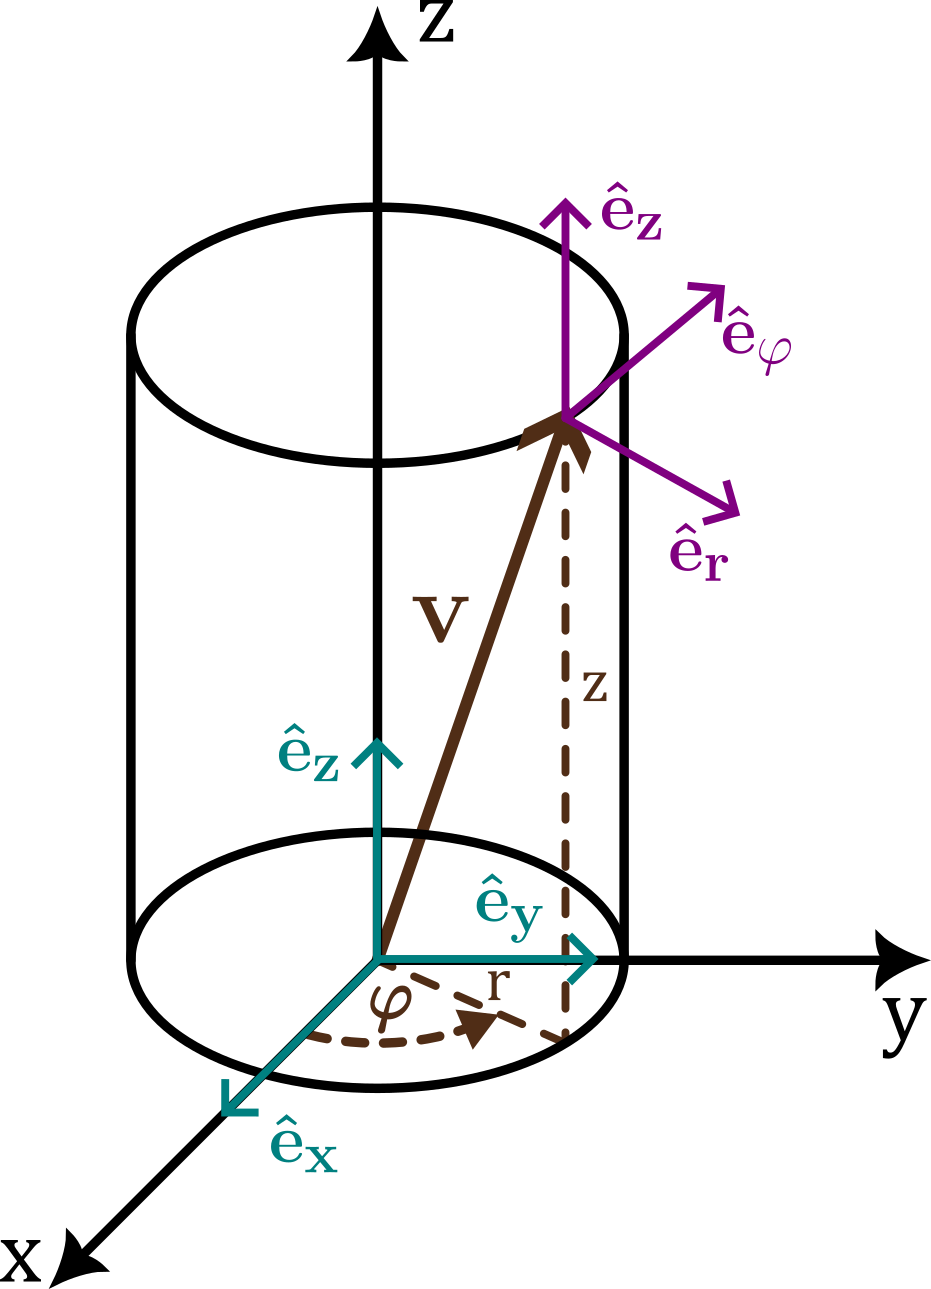
\includegraphics[width=0.5\textwidth]{figs/cylcoords}
    \caption{Cylindrical coordinates and their relationship to cartesian coordinates.}
    \label{fig:cylcoords}
\end{wrapfigure}

Where in cartesian coordinates we have
the basis vectors $\ex, \ey, \ez$
along the x, y and z axis, in cylindrical coordinates we have
$\er, \ephi, \ez$ as illustrated in
figure \ref{fig:cylcoords}. Note that $\er$ and $\ephi$
change direction depending on the current value of $\varphi$.

The basis vectors are related through the equations
\begin{align}
    \er   & = \cos(\varphi)\ex + \sin(\varphi)\ey  \\
    \ephi & = -\sin(\varphi)\ex + \cos(\varphi)\ey \\
    \ez   & = \ez
\end{align}

\subsubsection{Scaling Factors}
In cylindrical coordinates, scaling factors are needed for
common differential operators. For a scalar field $\Psi(r, \varphi, z)$
the gradient is defined as
\begin{equation}
    \nabla \Psi = \frac{\partial \Psi}{\partial r} \er +
    \frac{1}{r} \frac{\partial \Psi}{\partial \varphi} \ephi +
    \frac{\partial \Psi}{\partial z} \ez
    \label{eq:cylgrad}
\end{equation}

The divergence of a vector field $\vb{V}(r, \varphi, z)$ is
\begin{equation}
    \nabla \cdot \vb{V} = \frac{1}{r} \frac{\partial}{\partial r} (rV_r)
    + \frac{1}{r} \frac{\partial V_\varphi}{\partial \varphi}
    + \frac{\partial V_z}{\partial z}
    \label{eq:cyldiv}
\end{equation}
which gives the laplacian $\nabla^2 \Psi = \nabla \cdot \nabla \Psi (r, \varphi, z)$
\begin{equation}
    \nabla^2 \Psi =
    \frac{1}{r} \frac{\partial}{\partial r} \left(r\frac{\partial \Psi}{\partial}\right)
    + \frac{1}{r^2} \frac{\partial^2 \Psi}{\partial \varphi^2}
    + \frac{\partial^2 \Psi}{\partial z^2}
    \label{eq:cyl_laplacian}
\end{equation}
\cite[Ch.3.13]{russenschuck_field_2011}
\subsubsection{The Laplace Equation in Cylindrical Coordinates}
One way to solve the laplacian is to use separation of variables
technique to find the set of potential solutions, and from that
set choose the ones that make sense for our problem.

Firstly, we make the ansatz that the solutions can be written in
the form
\begin{equation}
    \Psi(r, \varphi, z) = R(r)\varPhi(\varphi)Z(z)
    \label{eq:psi_ansatz}
\end{equation}

Insertion of equation \ref{eq:psi_ansatz} into \ref{eq:cyl_laplacian}
then gives us
\begin{equation}
    \nabla^2 \Psi = \frac{1}{rR} \frac{d}{dr} \left(\frac{dR}{dr} \right)
    + \frac{1}{r^2 \varPhi} \frac{d^2 \varPhi}{d\varphi^2}
    + \frac{1}{Z} \frac{d^2 Z}{dz^2}
    \label{eq:sepLaplacian}
\end{equation}

We know from equation \ref{eq:laplacian_zero} that this is equal to zero,
and can therefore rewrite as
\begin{equation}
    -\frac{1}{\varPhi} \frac{d^2 \varPhi}{d\varphi^2} =
    \frac{r}{R} \frac{d}{dr} \left(\frac{dR}{dr} \right)
    + \frac{r^2}{Z} \frac{d^2 Z}{dz^2}
\end{equation}
Here, a contradiction emerges. A change in $\varphi$ can only
introduce a change in the left hand side of this equation. Likewise,
this equality must still hold for a change in $r$ or $z$. These
conditions only hold under the assumption that both sides are constant,
such that
\begin{equation}
    \frac{1}{\varPhi} \frac{d^2 \varPhi}{d\varphi^2} = \alpha_1
\end{equation}
where $\alpha_1$ is constant. Using similar reasoning for $Z(z)$
and then $R(r)$ we can reduce this partial differential equation to
a system of differential equations in one variable.
\begin{align}
    \frac{d^2R}{dr^2} + \frac{1}{r} \frac{dR}{dr} & =
    \left( \frac{\alpha_1}{r^2} + \alpha_2 \right)R
    \label{eq:diffeqR}                                                \\
    \frac{d^2 \varPhi}{d\varphi^2}                & = \alpha_1\varPhi
    \label{eq:diffeqPhi}                                              \\
    \frac{d^2 Z}{dz^2}                            & = \alpha_2 Z
    \label{eq:diffeqZ}
\end{align}

While the differential equations in $\varPhi$ and $Z$ have a well defined
set of solutions using elementary functions like sines, cosines and exponentials,
equation \ref*{eq:diffeqR} is a bit trickier. This equation is known as
the Bessel differential equation, and solving it will require a
set of functions known as the Bessel functions. \cite{weisstein_bessel_nodate}

\subsection{Bessel Functions}
The Bessel functions are defined as the solutions to equation \ref*{eq:diffeqR}.
They come in several different variants depending on the values of $\alpha_1$ and
$\alpha_2$. They are not expressible using elementary functions and must therefore
be approximated using for example, power series solutions, generating functions
or numeric integration.

The actual calculation of the Bessel functions is outside the scope of this thesis,
more than stating that they are implemented in most popular programming languages.
Still, a short overview of the properties of the most relevant subset of Bessel
functions will aid greatly in finding the solutions to our magnetic scalar potential.
\cite{weisstein_bessel_nodate}
\subsubsection{Bessel Function, First Kind}

The Bessel function of the first kind is a collection of functions that are nonsingular
at the origin. It is often denoted $\Jn{n}(x)$. Figure \ref*{fig:Jnplot} shows
$\Jn{n}(x)$ for $n=0,1,2,3,4$.

\begin{figure}[h]
    \centering
    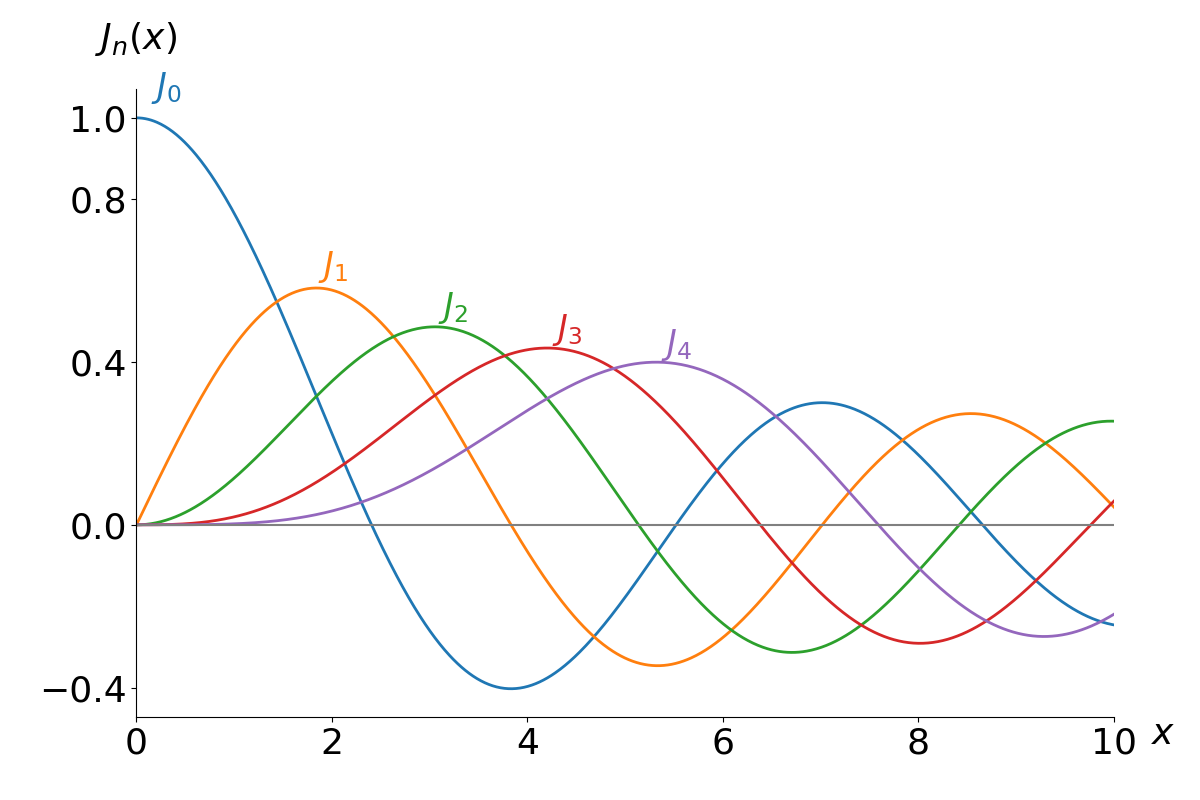
\includegraphics[width=0.7\textwidth]{figs/Jnplot.png}
    \caption{Bessel functions of the first kind, for $n\in[0,4]$.}
    \label{fig:Jnplot}
\end{figure}

For negative $n$ we have
\begin{equation}
    \Jn{-n}(x) = (-1)^n \Jn{n}(x)
\end{equation}

and for the first derivative of $\Jn{n}$ we have
\begin{equation}
    \Jn{n}' = \frac{1}{2}\left( \Jn{n-1} -  \Jn{n+1} \right)
\end{equation}

Another important property is
\begin{align}
    \Jn{0}(0) & = 1                                  \\
    \Jn{n}(0) & = 0, \, \forall n\in\mathbb{Z}/\{0\}
\end{align}
\cite{weisstein_bessel_nodate-2}
\subsubsection{Modified Bessel Function, First Kind}
For the Bessel function of the first kind with imaginary
arguments, the modified Bessel function $\In{n}(x)$ is often used.
It is related to the regular first kind Bessel function
through the equality
\begin{equation}
    \In{n}(x) = j^{-n}\Jn{n}(jx)
\end{equation}
\cite{weisstein_modified_nodate}
The first five terms of $\In{n}$ can be seen in figure \ref*{fig:Inplot}.

\begin{figure}[h]
    \centering
    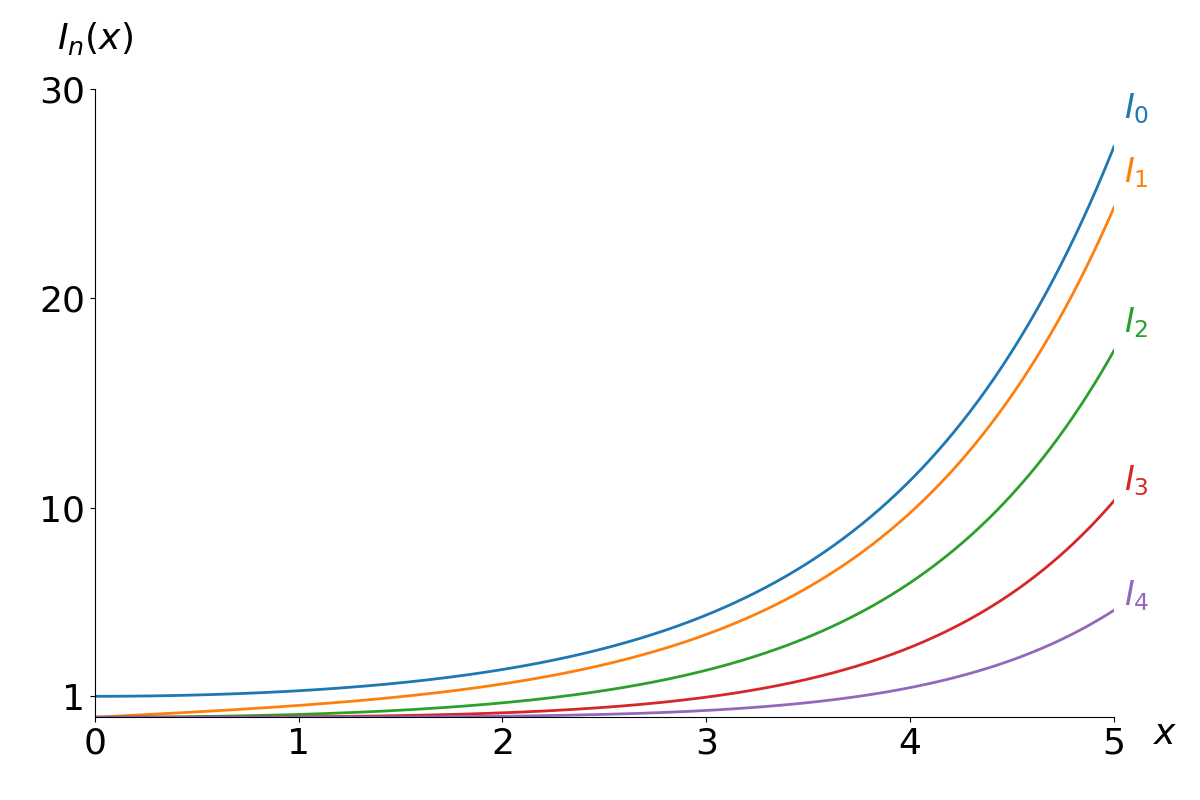
\includegraphics[width=0.7\textwidth]{figs/Inplot.png}
    \caption{Modified Bessel functions of the first kind, for $n\in[0,4]$.}
    \label{fig:Inplot}
\end{figure}

\subsubsection{Bessel Function, Second Kind}
The Bessel function of the second kind is a solution to
the Bessel differential equation that is singular at the
origin. It can be seen in figure \ref{fig:Ynplot}.\cite{weisstein_bessel_nodate-1}

\begin{figure}[h]
    \centering
    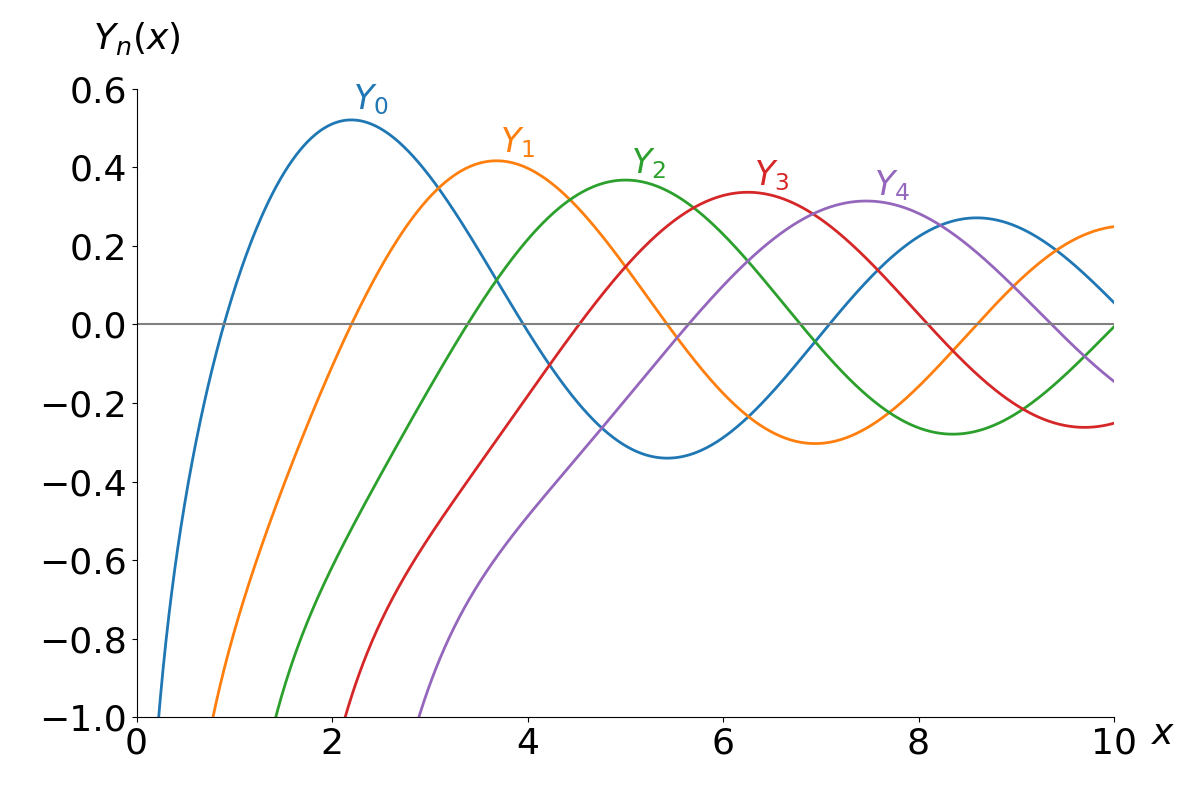
\includegraphics[width=0.7\textwidth]{figs/Ynplot.png}
    \caption{Bessel functions of the second kind, for $n\in[0,4]$.}
    \label{fig:Ynplot}
\end{figure}

\subsection{Bessel-Fourier-Fourier Series}
\label{subsec:BFF}
With the set of potential solutions to $\Psi(r,\varphi,z)$ established,
we can start to eliminate the impossible ones. The domain $\Omega$
is spanned by the magnetometer and its path along the z axis, making up
the cylindrical domain. Examples of this domain can be seen in figures
\ref{fig:aligned_domain} and \ref{fig:unaligned_domain}. Keep in mind
that the domain is always spanned by and relative to the magnetometer and
its path along z, and is thus the same regardless of the magnets
relative positioning to the PCB.
\begin{figure}[!h]
    \centering
    \begin{subfigure}[b]{0.45\textwidth}
        \centering
        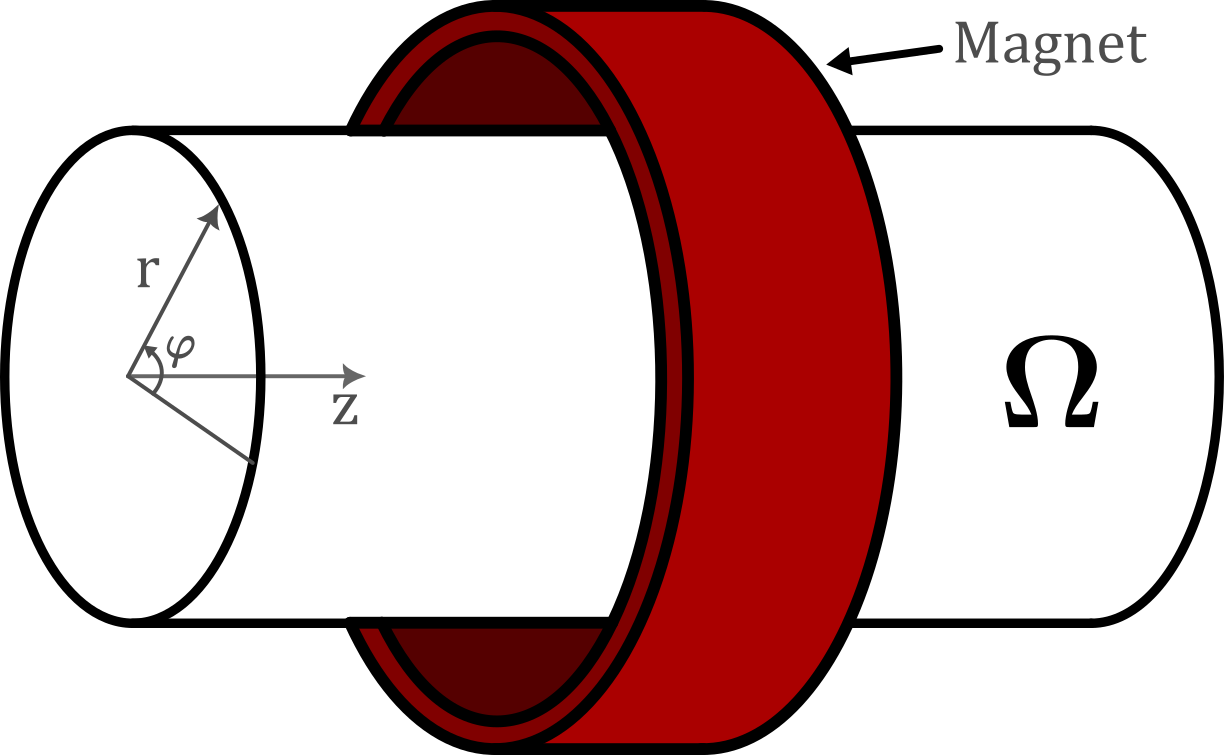
\includegraphics[width=0.9\textwidth]{figs/aligned_domain.png}
        \caption{The measurement domain $\Omega$
            inside the aperture of a solenoid.}
        \label{fig:aligned_domain}
    \end{subfigure}
    \hfill
    \begin{subfigure}[b]{0.45\textwidth}
        \centering
        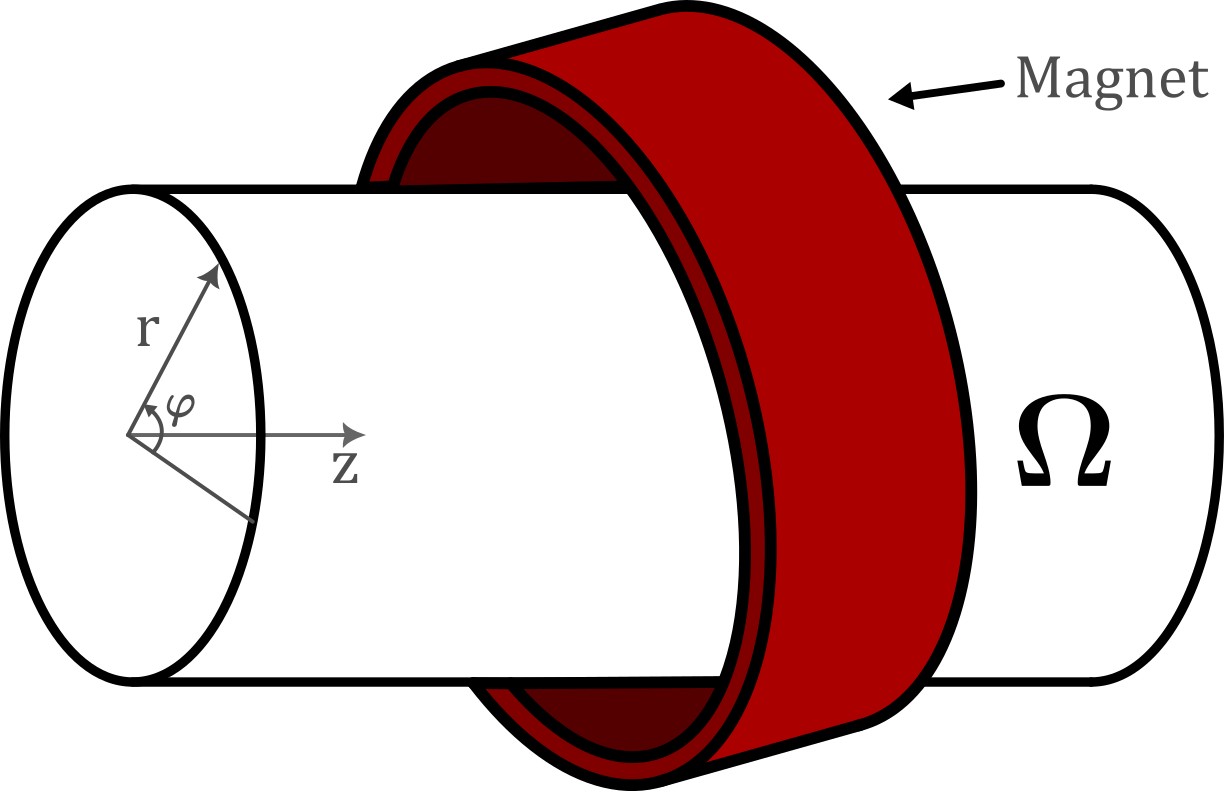
\includegraphics[width=0.9\textwidth]{figs/unaligned_domain.png}
        \caption{The measurement domain $\Omega$
            inside the aperture of an unaligned solenoid.}
        \label{fig:unaligned_domain}
    \end{subfigure}
\end{figure}
Using a table of known solutions to equations
\ref{eq:diffeqR}-\ref{eq:diffeqZ} from the book "Field theory handbook"
\cite{moon_field_1988} we can find the relevant ones.

\begin{align*}
    \frac{d^2R}{dr^2} + \frac{1}{r} \frac{dR}{dr} & =
    \left( \frac{\alpha_1}{r^2} + \alpha_2 \right)R
    \tag{\ref{eq:diffeqR} revisited}                                  \\
    \frac{d^2 \varPhi}{d\varphi^2}                & = \alpha_1\varPhi
    \tag{\ref{eq:diffeqPhi} revisited}                                \\
    \frac{d^2 Z}{dz^2}                            & = \alpha_2 Z
    \tag{\ref{eq:diffeqZ} revisited}
\end{align*}

Firstly, the measurements start and end far outside of the magnet,
where the field is negligibly close to zero. Thus, the sum of the solutions
in $z$ must start and end at zero. Since the solutions must be periodic
over the length of the domain, we have our first boundary condition
\begin{align}
    qkz  & = \frac{2\pi}{L}kz, \,k\in\mathbb{N}_1 \\
    Z(z) & = 0\text{ if } z\in\{0,L\}
\end{align}
where $-(qk)^2 = \alpha_2$ and $L$ is the length of the domain in z.

A Fourier series is a solution.
\begin{equation}
    Z(z) = \sum\limits_{k=1}^{\infty}
    \mathfrak{A}_k\sin{(qkz)} + \mathfrak{B}_k\cos{(qkz)}
\end{equation}
where $\mathfrak{A, B}$ are as of yet unknown coefficients.

Secondly, since $\varPhi(\varphi)$ spans the whole circumference of
$\Omega$, and the field is continuous inside the domain, we have
our next boundary condition

\begin{equation}
    \varPhi(0) = \varPhi(2\pi)
\end{equation}

Once again, a Fourier series is a solution
\begin{equation}
    \varPhi(\varphi) = \sum\limits_{n=1}^{\infty}
    \mathfrak{D}_n\sin{(n\varphi)} + \mathfrak{E}_n\cos{(n\varphi)}
    , \, n\in\mathbb{N}_1
\end{equation}
giving us $\alpha_1 = -n^2$.

With both $\alpha_1$ and $\alpha_2$ found, $R(r)$ in equation \ref{eq:diffeqR}
is now completely determined as
\begin{equation}
    R(r) = \sum\limits_{k=0}^{\infty}
    \mathfrak{F}_{k}\Jn{n}(jqkr) + \mathfrak{G}_k\Yn{n}(jqkr)
\end{equation}
Since we know that the magnetic field is not singular inside the aperture
(Biot Savart, equation \ref{eq:Biot_Savart} gives us singularities only inside
the current carrying wires.) we can immediately discard $\Yn{n}$ as potential
solution. Since the argument for $\Jn{n}$ is imaginary, we can also substitute
with the modified Bessel function of the first kind, giving us
\begin{equation}
    R(r) = \sum\limits_{k=1}^{\infty}
    j^{-k}\mathfrak{F}_{k}\In{n}(qkr)
\end{equation}

We still need to account for the fact that the $\vb{B}$-field might have
a non zero mean over the domain, i.e. adding the zero terms of the series.
For $Z(z)$, this is simply

\begin{equation}
    Z(z) = \mathfrak{A}_{0,0}z
\end{equation}

while in $r$ this will be
\begin{equation}
    R(r) = \sum\limits_{n=1}^{\infty} \mathfrak{F}_{n,0}r^n
\end{equation}
\cite[pp.12-14]{moon_field_1988}
The $n=0$ terms for $R(r)$ and $\varPhi(\varphi)$ have been discarded,
as that would be equivalent to a magnetic monopole, which have never
been found experimentally, and is unlikely to be found using a simple
solenoid magnet.\cite{acharya_search_2022}

Now, all the potential solutions can be combined into one double
series. By also converting the Fourier series from real to complex
valued double sided series, we can combine the
$\mathfrak{A, B, D, E \text{ and } F}$
coefficients into one complex valued coefficient $\Cnk$. The values
of these coefficients are unknown until fitted to measurements or
calculated. For known coefficients, instead $C_{n,k}$ will be used.
The permittivity constant $\mu_0$ will hereafter be baked into the
coefficients.

After a lot of algebra, this yields
\begin{equation} \label{eq:Psi}
    \begin{split}
        \Psi(r,\varphi,z) &=\Cnk[0,0]z + \Bffok +\\
        &+ \Bffno +\\ &+ \Bffnk
    \end{split}
\end{equation}

Technically, the first, second and fourth summands
can be merged into one sum, they are however separated
to make the distinction of the fundamental fourier series
in z and the higher order harmonics clearer.

It is worth noting that the third summand in the above series
are a commonly used form of two dimensional multipoles at CERN.
These are mainly used for dipole, quadropole, sextupole and
higher order magnets with no or very little B-field
derivative along the z axis inside the aperture.
\cite[Ch.6.1]{russenschuck_field_2011}

\subsection{Fundamentals and Harmonics of the BFF Series.}
As stated at the end of section \ref{sec:series_decompositions},
the $\vb{B}$ field components can be found by taking
the partial derivatives of our scalar potential in
equation \ref{eq:Psi}.
The $B_z$ component will then be
\begin{equation}
    \begin{split}
        B_z &= \frac{\partial \Psi}{\partial z} =
        \Cnk[0,0] + \Bffzok +\\
        &+ \Bffznk
    \end{split}
\end{equation}

while in $r$ we have
\begin{equation}
    \begin{split}
        B_r &= \frac{\partial \Psi}{\partial r} =
        \Bffrok + \\ &+ \Bffrno \\ &+\Bffrnk
    \end{split}
\end{equation}

and finally, in $\varphi$
\begin{equation}
    \begin{split}
        B_\varphi &= \frac{1}{r}
        \frac{\partial \Psi}{\partial \varphi} = \Bffpno +\\
        &+ \Bffpnk
    \end{split}
\end{equation}

We will now study the individual harmonics in $n$ of the
BFF series. First, it might be beneficial to give them
names for reference. Using the notation $\Psi_{n,k}$
for the harmonics, we have

\begin{table}[!h]
    \centering
    \begin{tabular}{l c p{2cm}}
        $\Psi_{n,k}$ & Summand         & Name                       \\ \hline
        1. $\Psi_{0,0}$ & $\Cnk[0,0]z$ & Dipole in $z$              \\
        2. $\Psi_{0,k}$ & $\Bffok$     & Solenoid Fundamentals      \\
        3. $\Psi_{n,0}$ & $\Bffno$     & Multipoles in $r, \varphi$ \\
        4. $\Psi_{n,k}$ & $\Bffnk$     & Solenoid Harmonics
    \end{tabular}
    \caption{Components of the Bessel-Fourier-Fourier Series.}
    \label{tab:BFF-components}
\end{table}

Using numerical calculations from a simple current loop
Biot-Savart model, the BFF series was fitted to $\vb{B}$
field points inside a cylindrical domain. The procedure
for this fitting is described in section \ref{sec:BFF-fitting}.
With this fitting, we can easily obtain field distributions of
the individual harmonics. Here, only the first two
harmonics $n\in\{0,1\}$ will be shown.

\subsubsection{Dipole in $z$}
The most fundamental part of the BFF series, this component
is a constant field tangential to $\ez$. This component
only exists for the $B_z$ field. A field map can
be seen in the figure below, with the arrows representing
direction of the field and the color the intensity. Colder
colors represent lower intensity and warmer colors higher
intensity.

\begin{figure}[h]
    \label{fig:zdip}
    \centering
    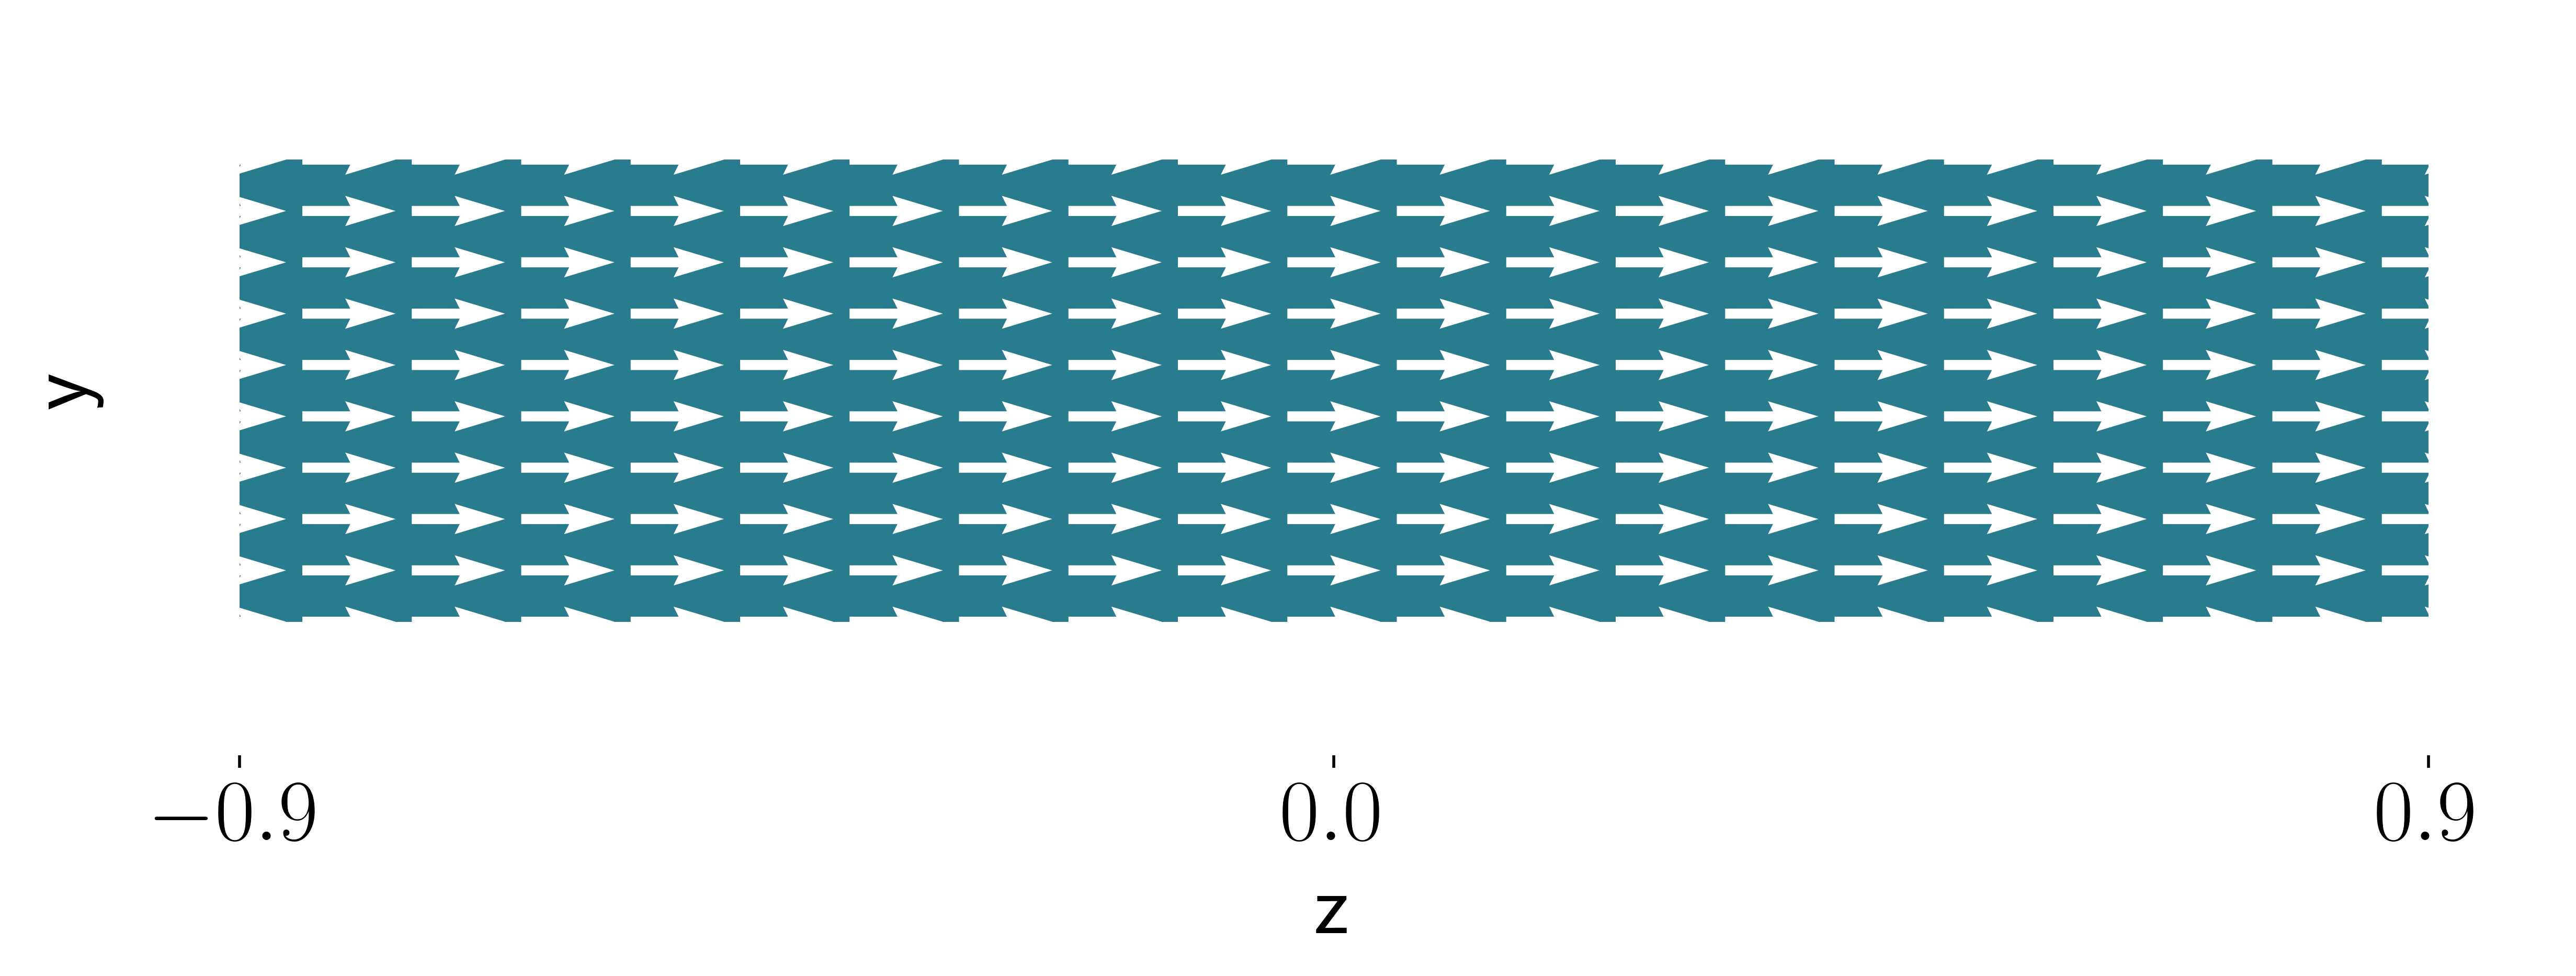
\includegraphics[width=0.8\textwidth]{figs/zdip.png}
    \caption{Field distribution of the dipole in $z$}
\end{figure}

\subsubsection{Solenoid Fundamentals}
The solenoid fundamentals describes the most basic solenoid
field, with no dependence on $\varphi$. The field is
perfectly symmetrical latitudinally around the $z$ axis, as
seen in figure \ref{fig:solfun} 

\begin{figure}[h]
    \centering
    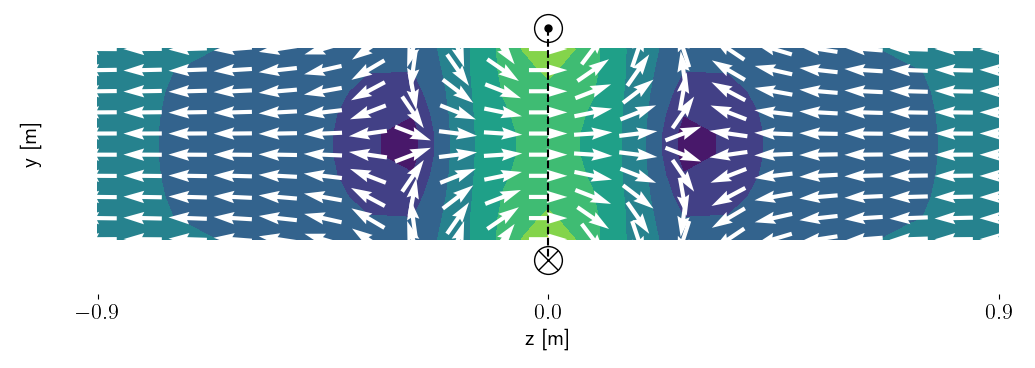
\includegraphics[width=0.8\textwidth]{figs/solfun.png}
    \caption{Field distribution of the solenoid fundamentals}
    \label{fig:solfun}
\end{figure}

The solenoid fundamentals along with the dipole in $z$ are
sufficient to describe an ideal solenoid field. They are
plotted together in figure \ref{fig:solfundip}

\begin{figure}[h]
    \centering
    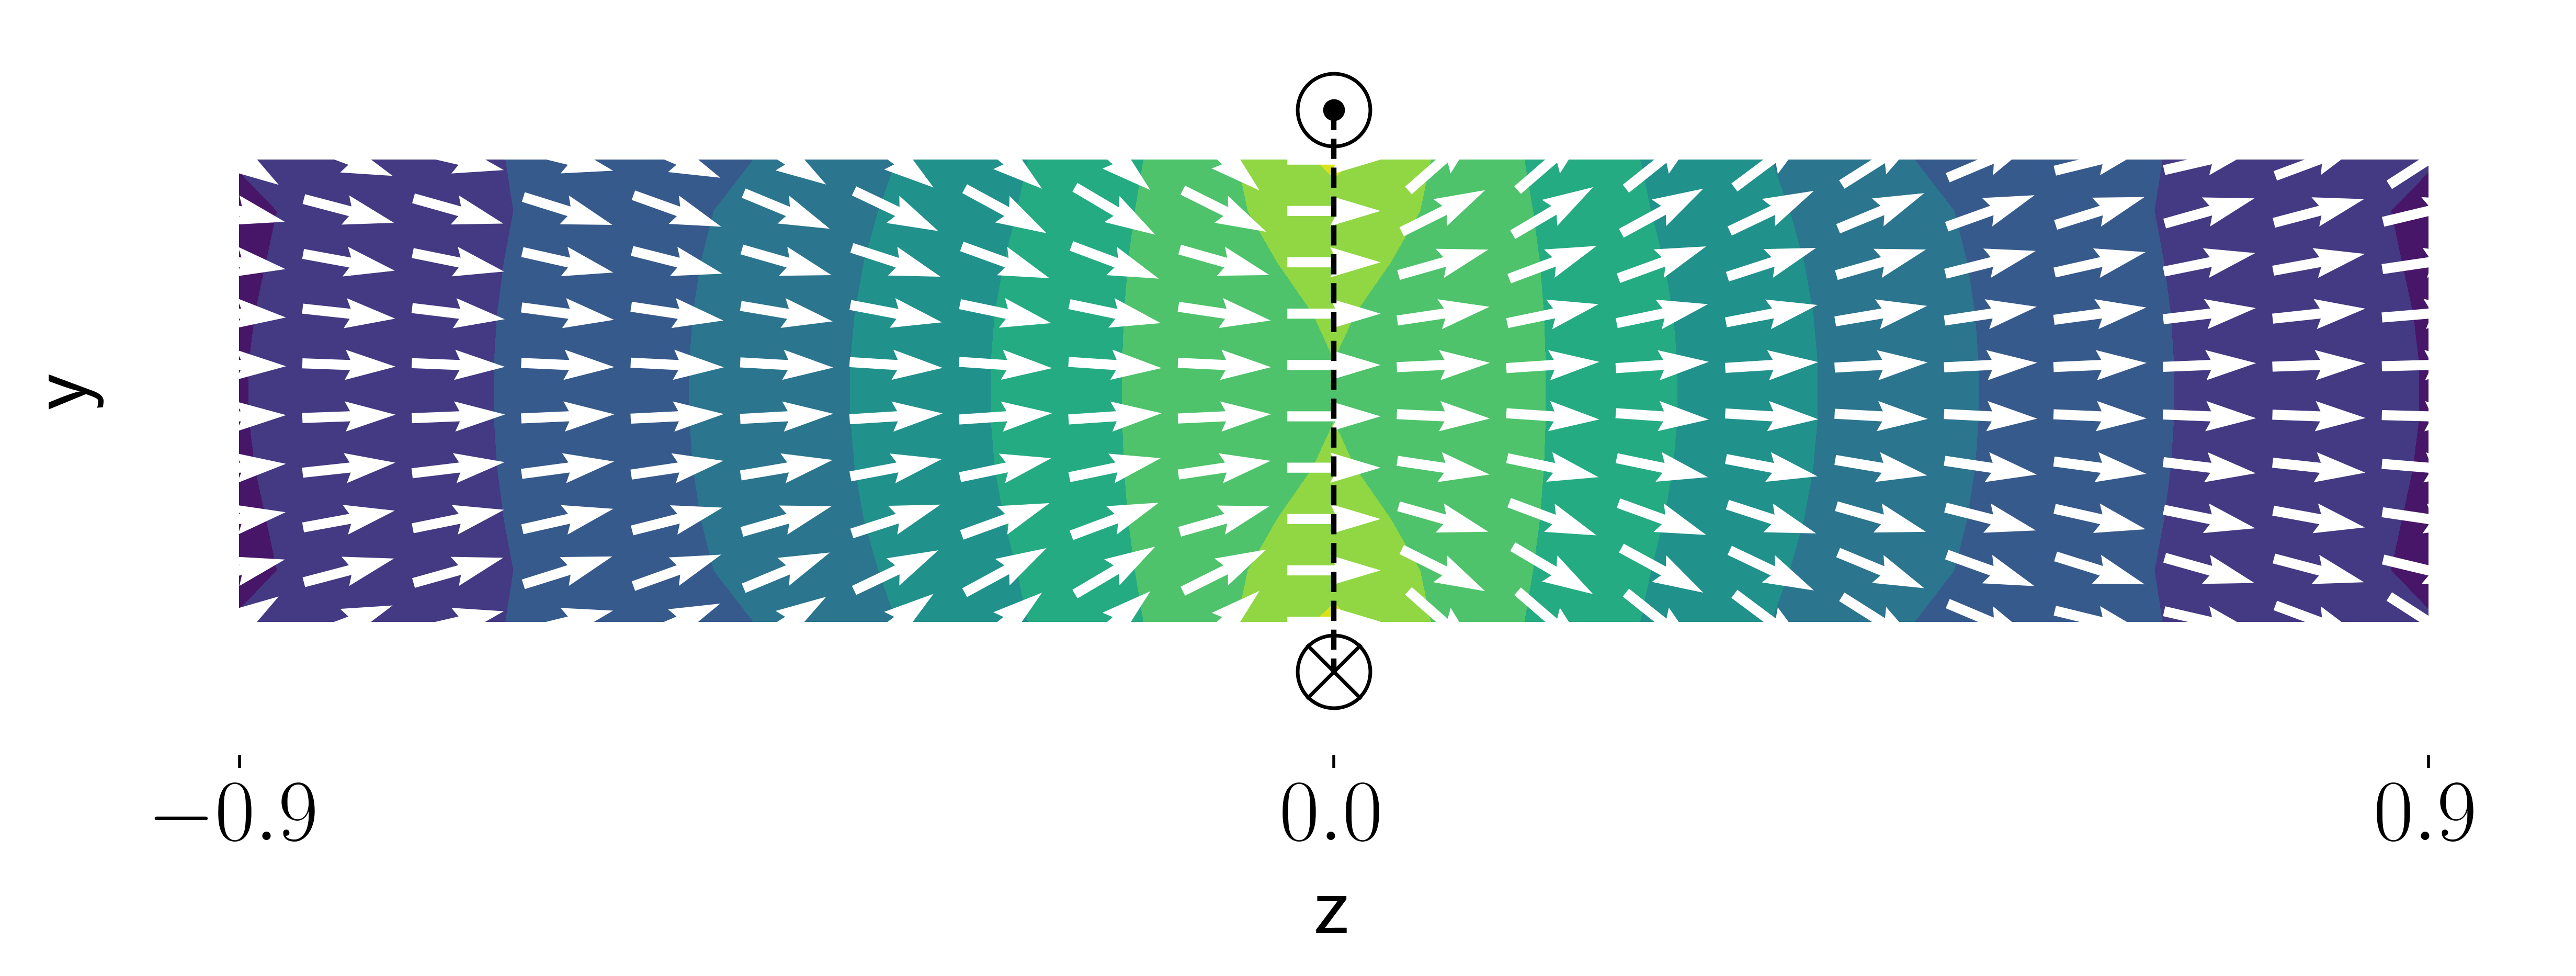
\includegraphics[width=0.8\textwidth]{figs/solfundip.png}
    \caption{Field map of an ideal solenoid field.}
    \label{fig:solfundip}
\end{figure}

The $z$ dipole can be thought of as the mean of the $Bz$
component, as illustrated in figure \ref{fig:solfundipplot}.

\begin{figure}[!h]
    \centering
    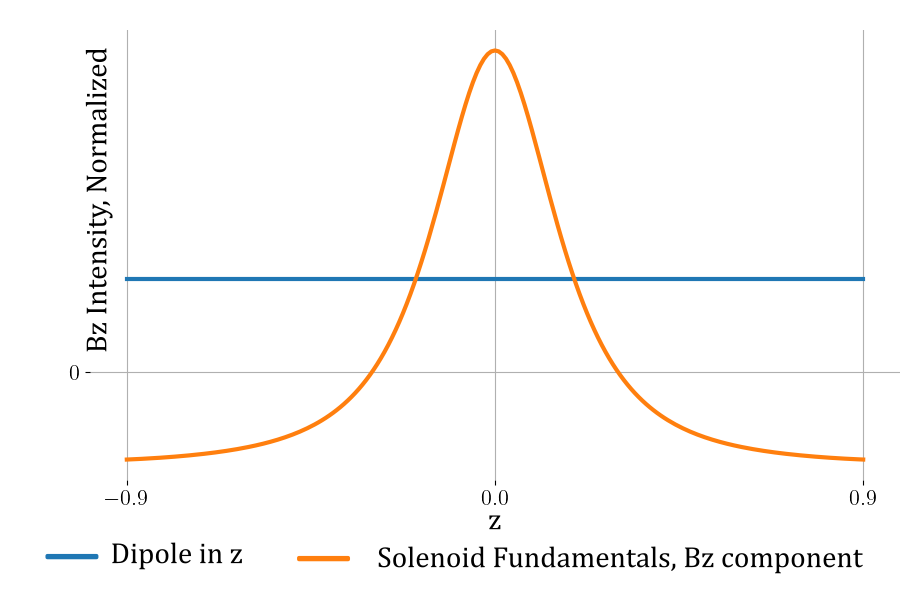
\includegraphics[width=0.8\textwidth]{figs/solfundipplot.png}
    \caption{$Bz$ field along the z axis.}
    \label{fig:solfundipplot}
\end{figure}

\subsubsection{Multipoles in $r, \varphi$}
As we move away from ideal solenoids to non ideal ones,
higher order harmonics must be introduced. For instance,
if the solenoid axis and the $z$ axis in our domain $\Omega$
are not perfectly parallel, the dipole moment of the solenoid
will be decomposed into two to three separate dipoles in
$r, \varphi$ and $z$ (or $x,y,z$ in cartesian coordinates).
This phenomena is illustrated in figure \ref{fig:rphidip}
for $n=1$ (dipole moment in $r, \varphi$) and a
magnet-domain pitch rotation of 0.3 radians.

\begin{figure}[!h]
    \centering
    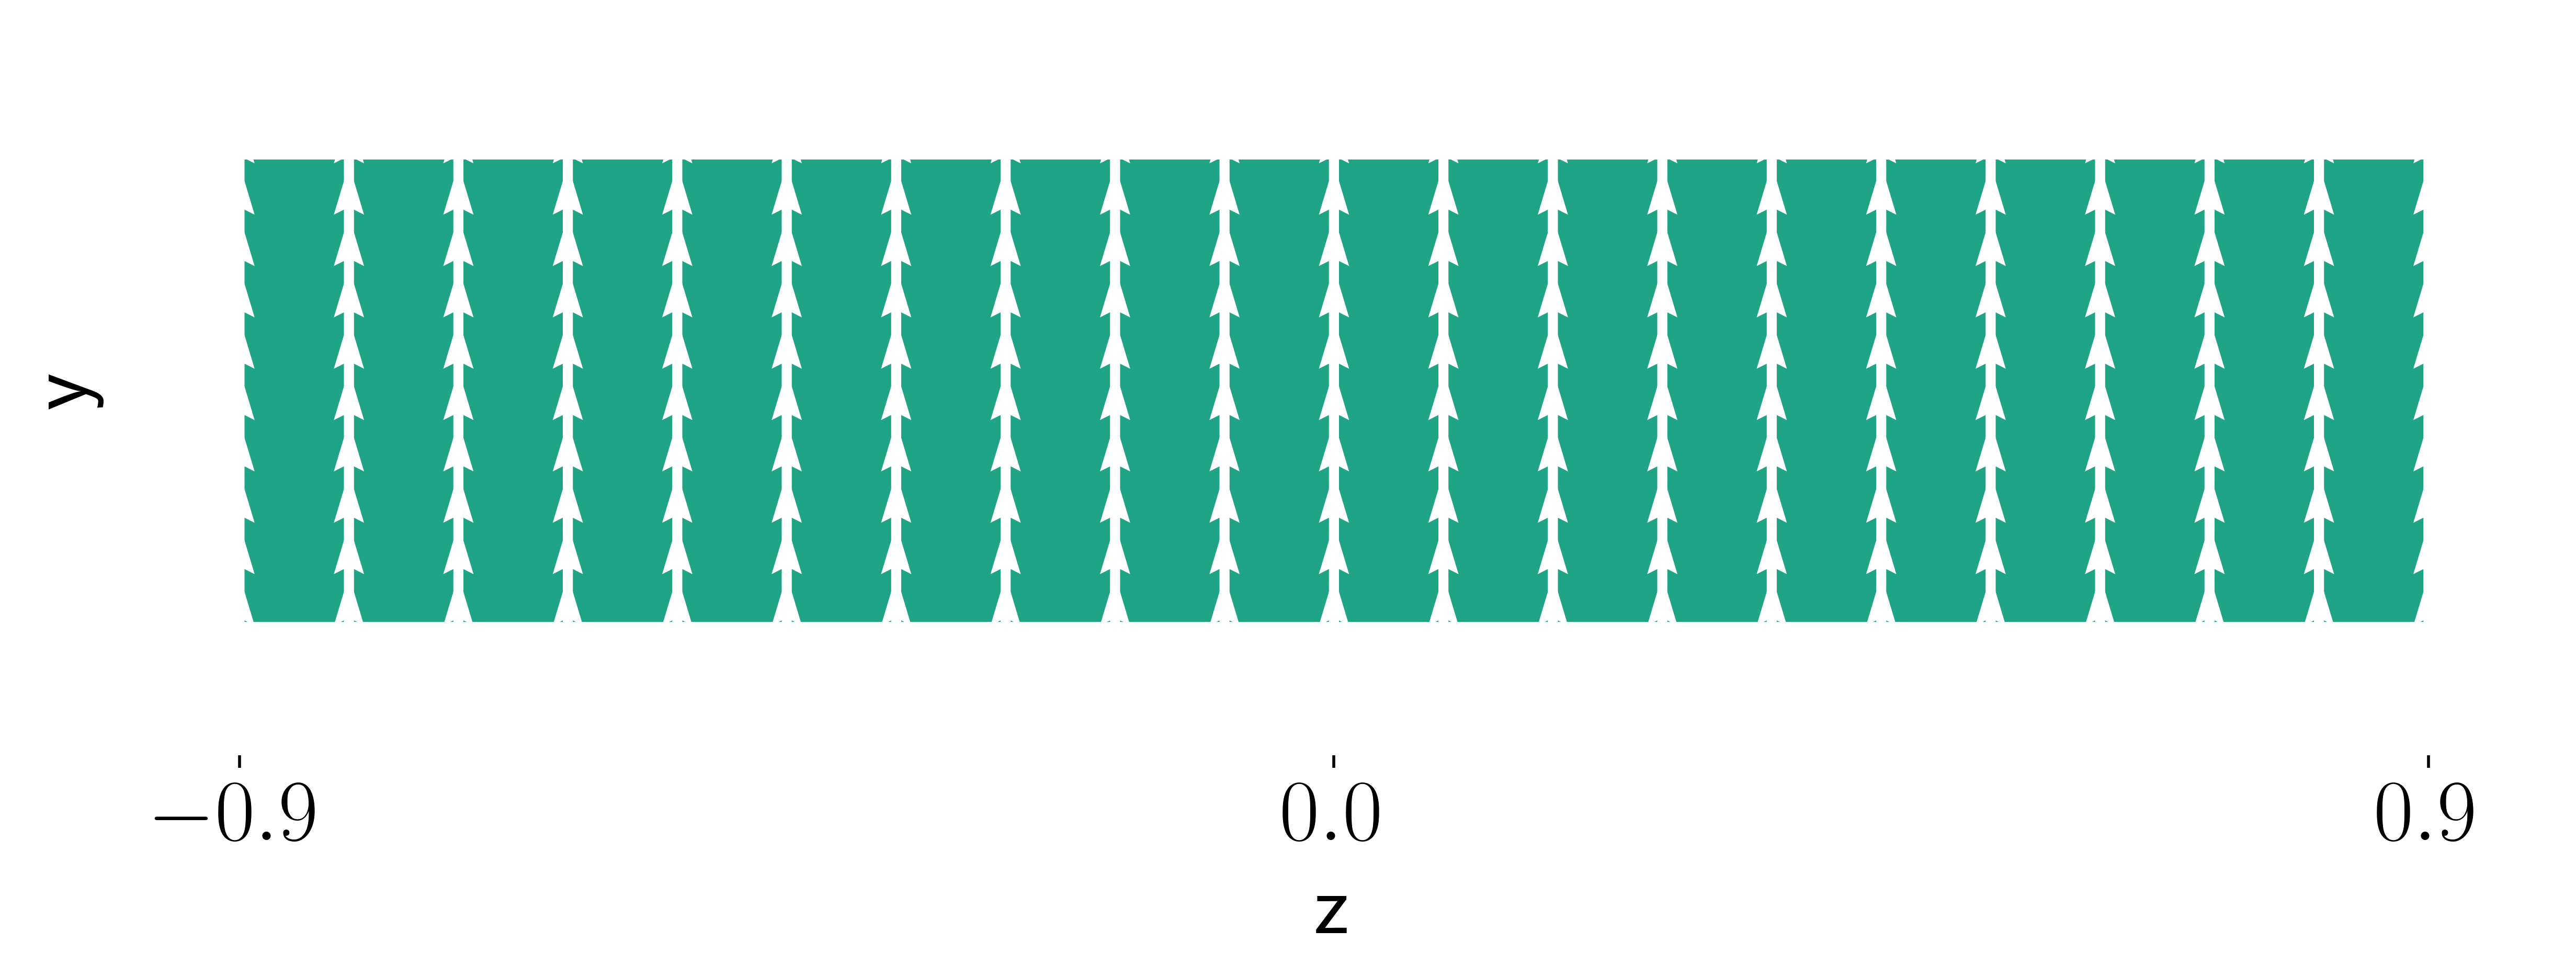
\includegraphics[width=0.8\textwidth]{figs/rphidip.png}
    \caption{Field distribution of the dipole in $r$, $\varphi$}
    \label{fig:rphidip}
\end{figure}

For higher orders of $n$, we will get the quadropoles, sextupoles
and so on in $r$ and $\varphi$.

\subsubsection{Solenoid Harmonics}
\label{subsubsection:solenoid-harmonics}
The solenoid harmonics throws a fourier series in
$\varphi$ into the mix. We can now represent fields that
are varying along the circumference of our cylindrical domain.

\begin{figure}[!h]
    \centering
    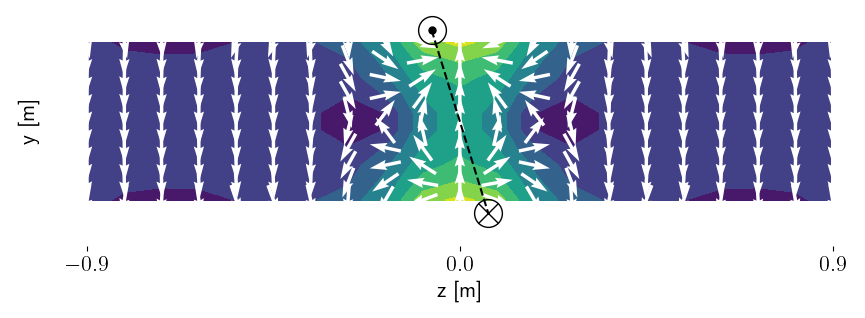
\includegraphics[width=0.8\textwidth]{figs/solharm.png}
    \caption{Field distribution of the solenoid harmonics.}
    \label{fig:solharm}
\end{figure}

Using all of the components together, we can get an accurate
field description of non ideal solenoid fields, as seen in figure
\ref{fig:allharmonics} for a domain that is tilted relative to the
magnet.

\begin{figure}[!h]
    \centering
    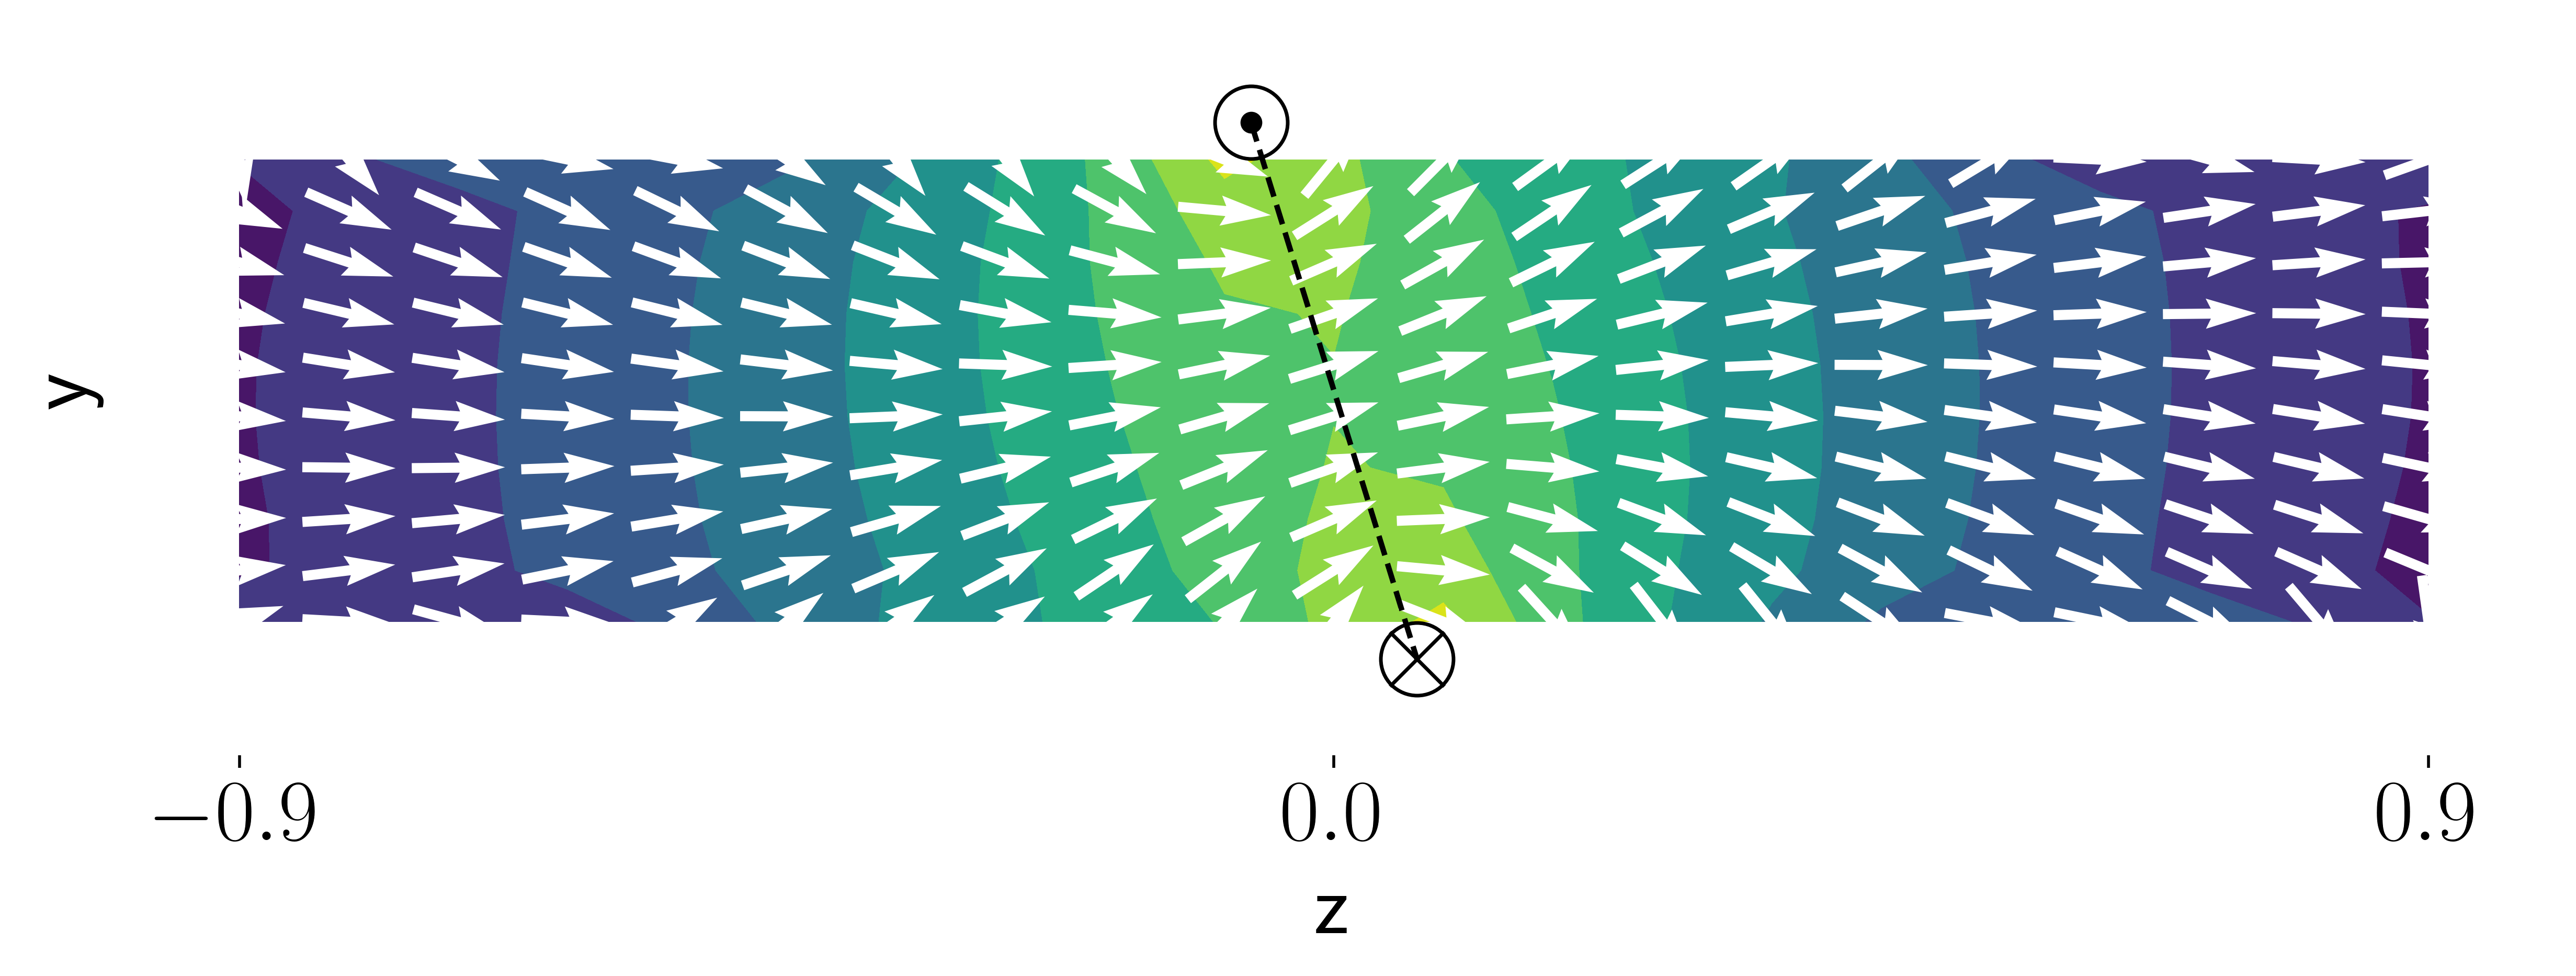
\includegraphics[width=0.8\textwidth]{figs/allcomponents.png}
    \caption{Field map of all BFF series components.}
    \label{fig:allharmonics}
\end{figure}

Just as with the dipole in $z$, the dipoles in $r,\varphi$
can be thought of as the mean of $B_r$ and $B_\varphi$
components.
This is illustrated in figure \ref{fig:radialplot}.

\begin{figure}[!h]
    \centering
    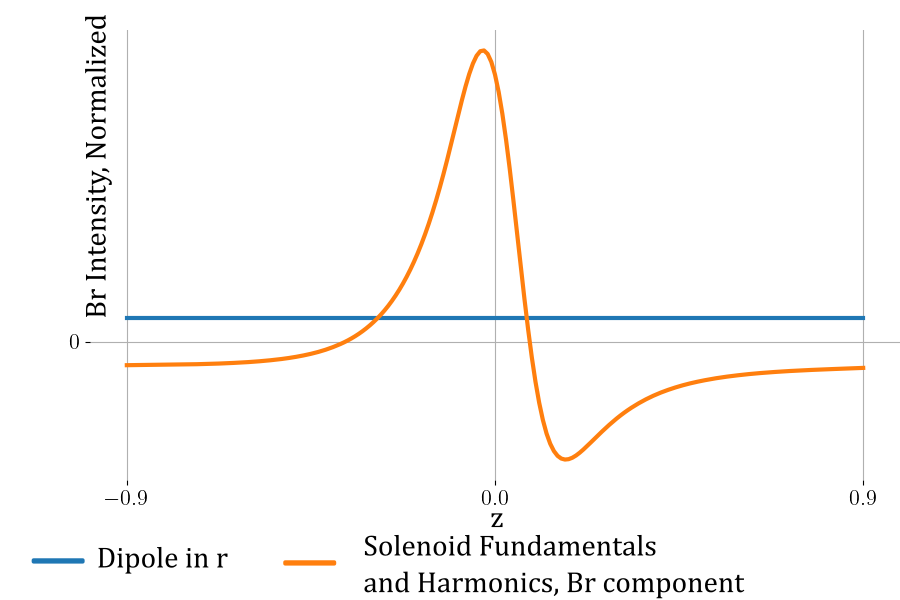
\includegraphics[width=0.8\textwidth]{figs/radialplot.png}
    \caption{Radial field along the $z$ axis, converted
        to cartesian coordinates.}
    \label{fig:radialplot}
\end{figure}

When a pitch or yaw angle rotation is present between the solenoid and
the domain, a "peak shift" between measurements of the $B_z$
field will be introduced, if the measurements are taken at
different longitudinal coordinates from the z-axis.
This is because of the higher order harmonics. The $n=0$ fundamentals will
not see this peak shift. They are invariant in $\varphi$,
as seen in figure \ref{fig:harmonicsskew}
\begin{figure}[!h]
    \centering
    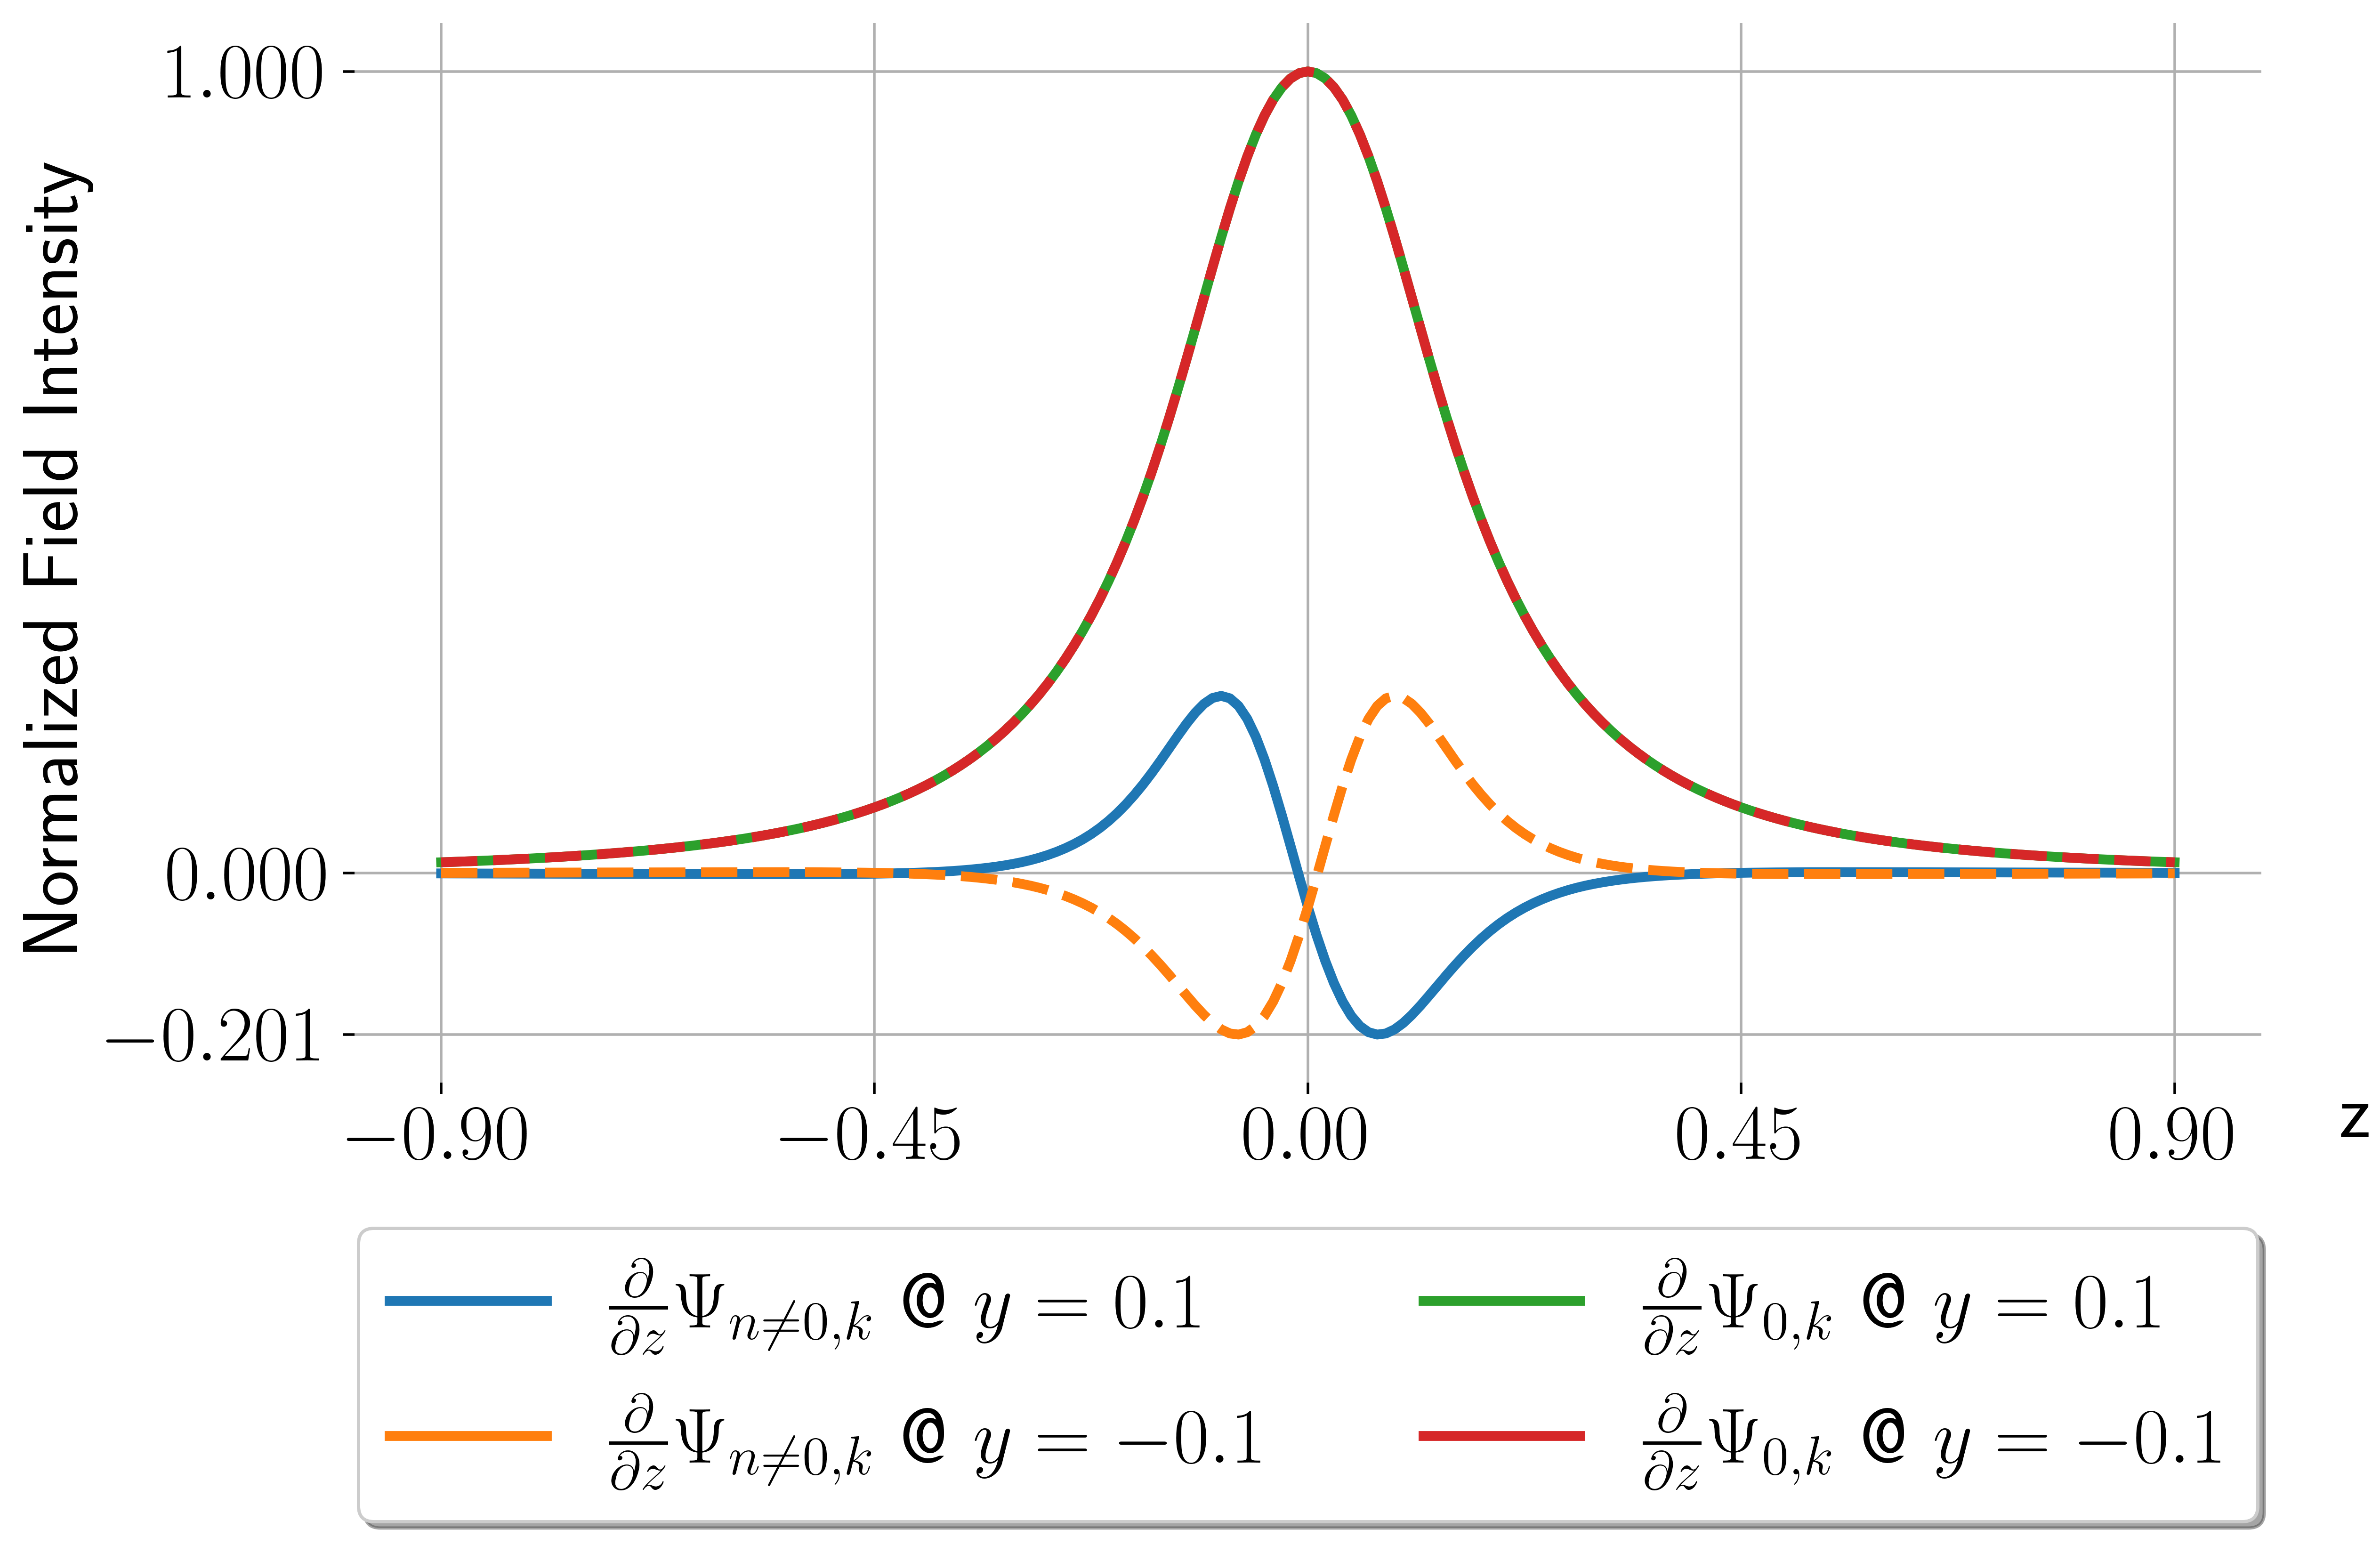
\includegraphics[width=0.8\textwidth]{figs/harmonicsskew.png}
    \caption{Different $B_z$ harmonics and their field distribution at
        different $y$ offsets for a tilted magnet.}
    \label{fig:harmonicsskew}
\end{figure}

When we add these skewed and non skewed harmonics together, we get the
aforementioned peak shift, which can be seen in figure \ref{fig:mirrored}.

\begin{figure}[!h]
    \centering
    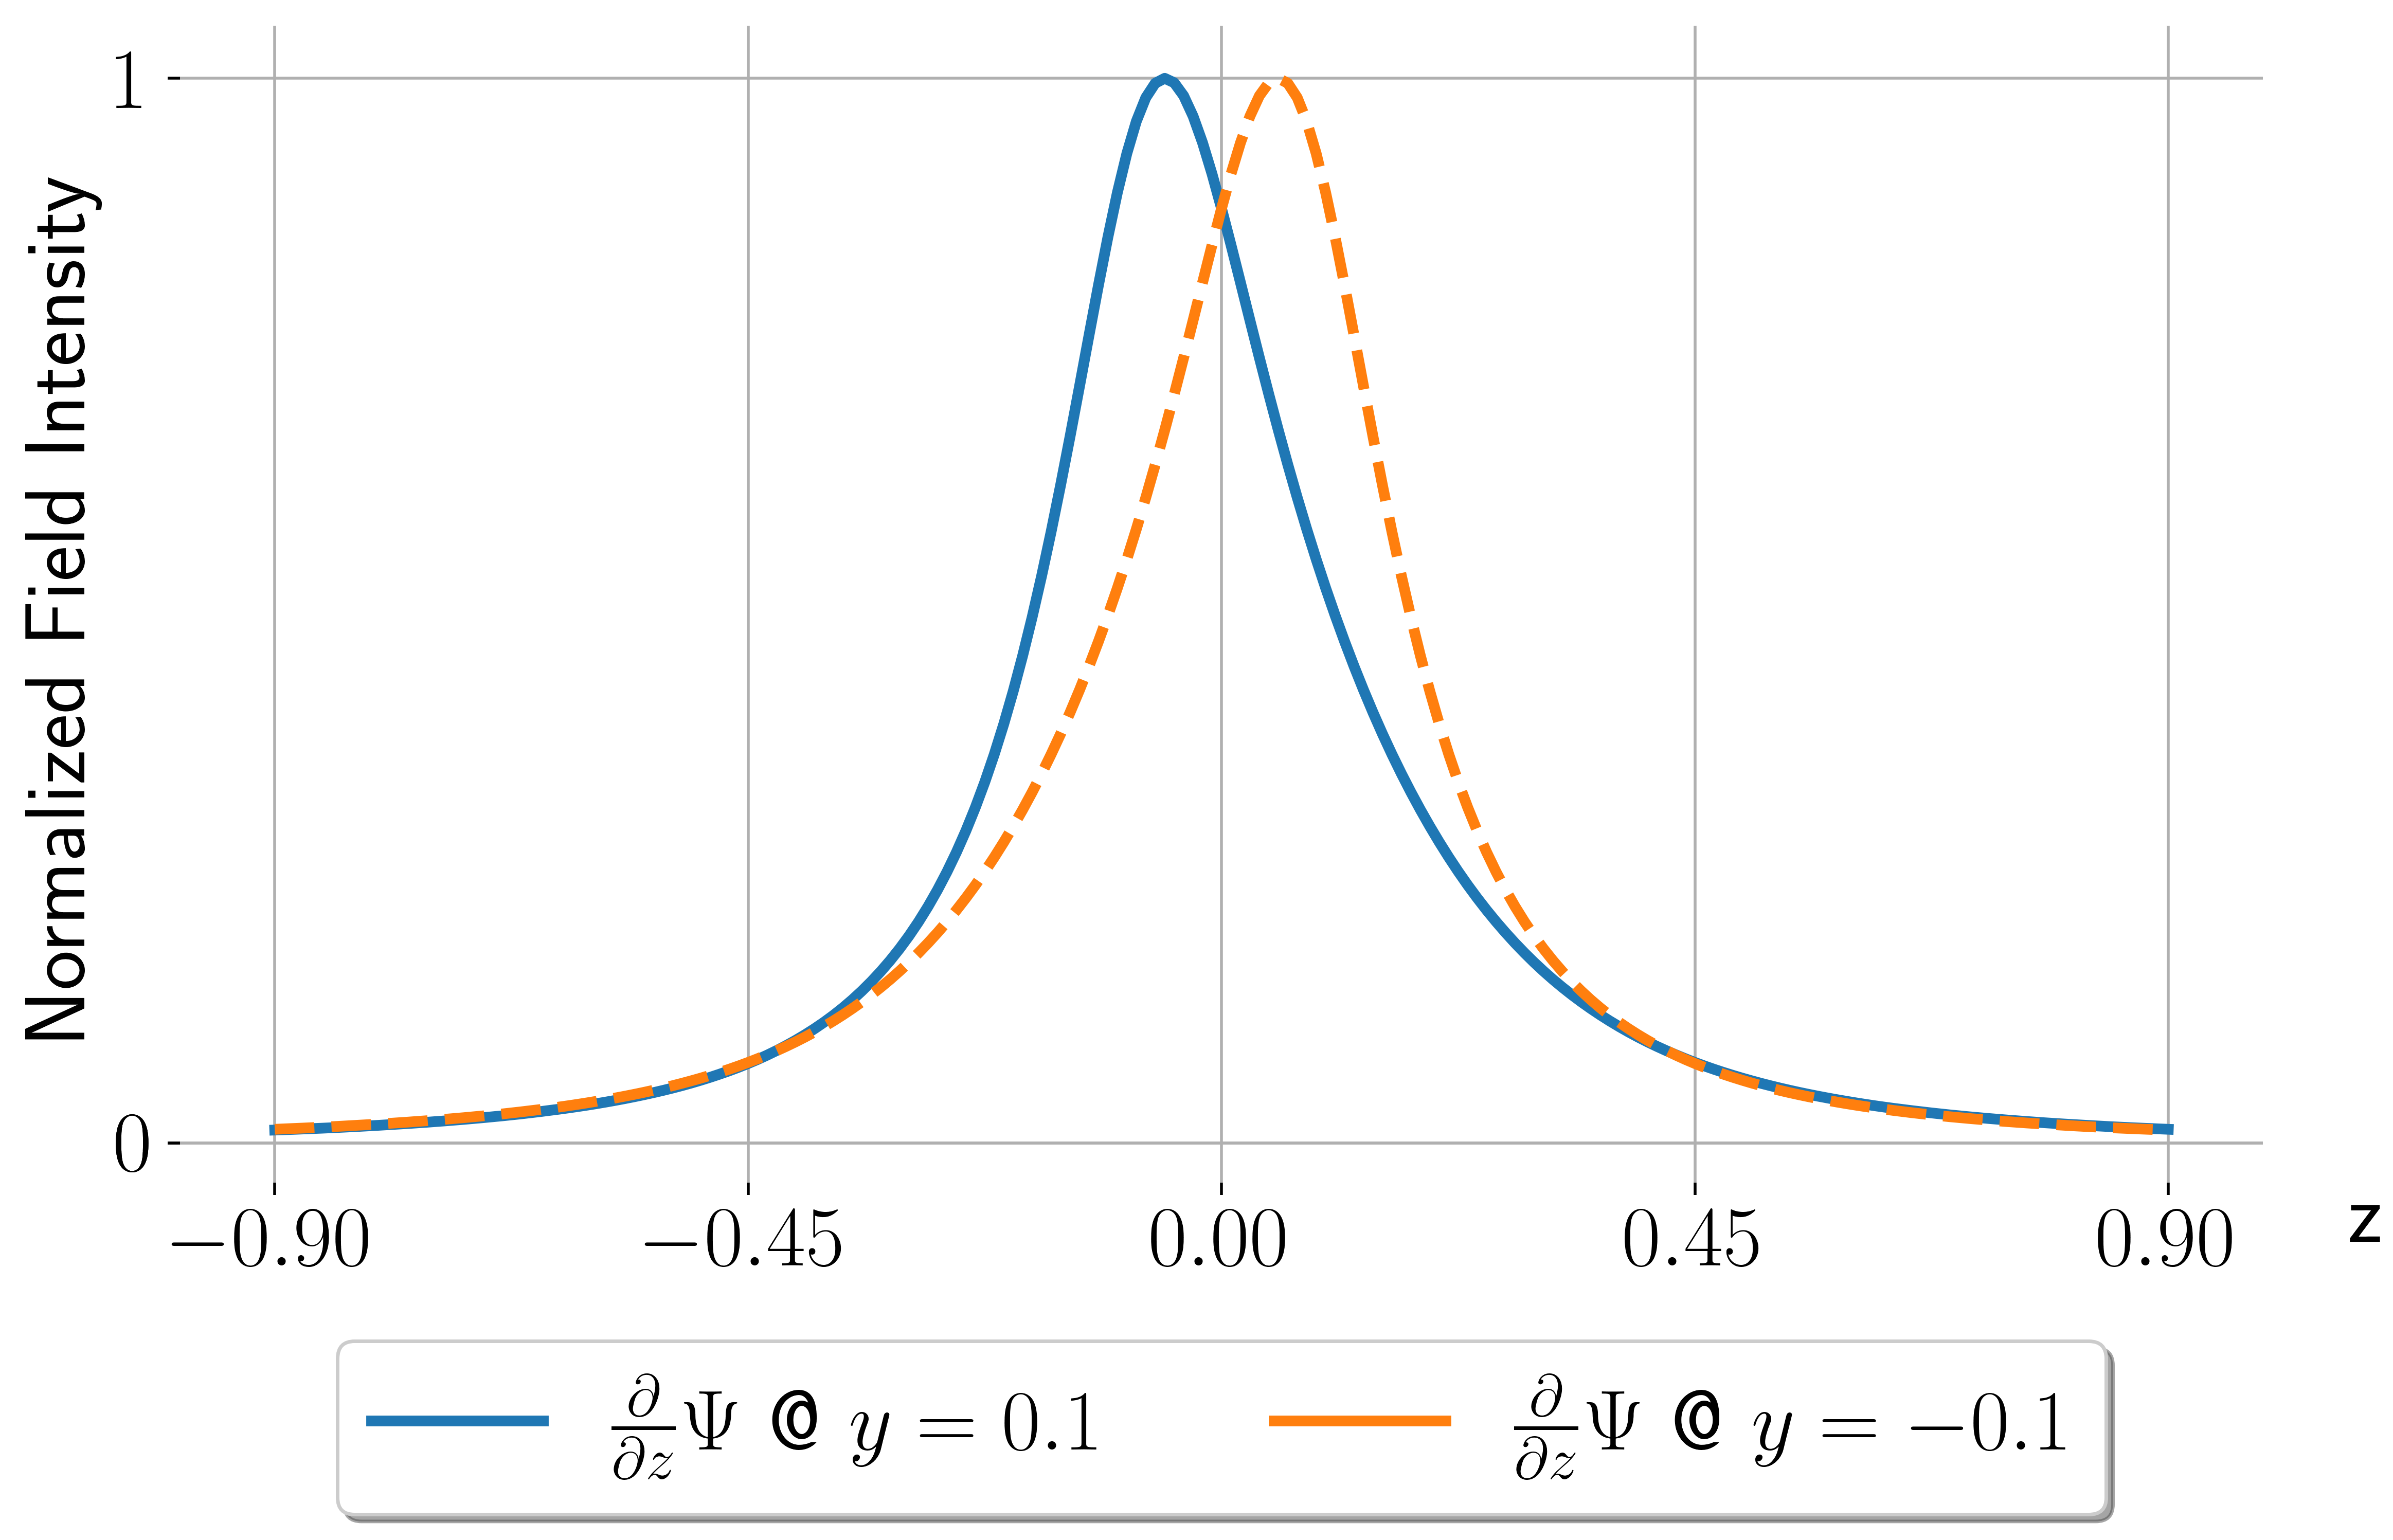
\includegraphics[width=0.8\textwidth]{figs/mirrored}
    \caption{Peak shifts for the $B_z$ field at opposite longitudinal
        coordinates, when the magnet has a pitch angle relative
        to the domain.}
    \label{fig:mirrored}
\end{figure}

To best measure how much a given field deviates from an ideal solenoid,
any measurement system must be designed such that it can capture the
higher order harmonics in $n$.

\FloatBarrier
\subsection{Dipole Components and the Integrated Field}
\label{sec:theory-dipoles}
By using Stokes theorem on equation \ref{eq:maxwell2}, one gets Amperes Law
in integral form,
\begin{equation}
    \oint \limits_C \vb{B} \cdot d\vb{l} =
    \mu_0 \iint\limits_S \vb{J}\cdot d\vb{S} = \mu_0 NI
    \label{eq:amperelaw}
\end{equation}
where the surface integral of the current density can be replaced
with the number of turns $N$ times the enclosed current $I$. $S$ is a surface enclosing
the current density $\vb{J}$ and $C$ is the boundary of $S$. $\vb{l}$
is parametrized curve describing C.
Now consider figure \ref{fig:ampereloop}.

\begin{figure}[!h]
    \centering
    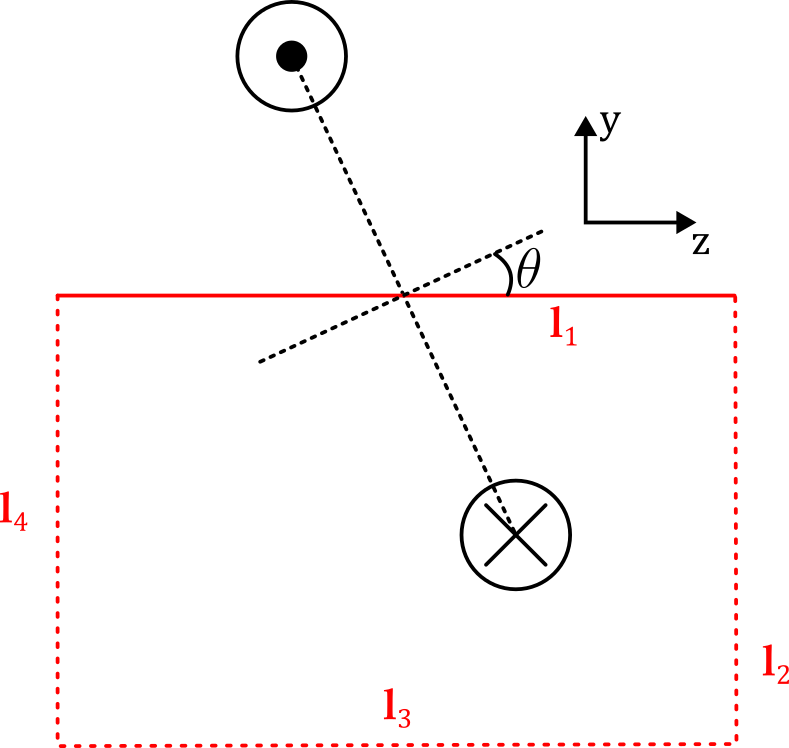
\includegraphics[width=0.7\textwidth]{figs/ampereloop}
    \caption{An amperian loop in a simple current loop.}
    \label{fig:ampereloop}
\end{figure}

Let $\vb{l}$ be the the concatenation of the curves
$\vb{l}_1,\vb{l}_2,\vb{l}_3,\vb{l}_4 $, whose images are straight
lines, and encloses
one end of a simple current loop. The axis of the current loop
has some angle $-\pi < \theta < \pi$ relative to the coordinate system.
If $\vb{l}_1$ and $\vb{l}_{2,4}$ are sufficiently long, such that their
ends are far out in the zero field, then the field at
the remaining lines $\vb{l}_{2,3,4}$ will also be
very close to zero. A good approximation of equation \ref{eq:amperelaw}
is then

\begin{equation}
    \int \limits_{\vb{l_1}} \vb{B}\cdot d\vb{l_1} \approx \mu_0 NI.
    \label{eq:amperian-line}
\end{equation}

Let $\vb{B}$ be described by the Bessel-Fourier-Fourier series $\Psi$,
with $\vb{l}_1$ spanning the length of the domain. Since $\Psi$ is
periodic in the length of the domain, all higher order components will
vanish in the integral and \ref{eq:amperian-line} becomes

\begin{equation}
    \int \limits_{\vb{l_1}} \frac{\partial\Psi}{\partial z} d\vb{l_1}
    = \int \limits_{-L/2}^{L/2} C_{0,0} dz = C_{0,0} L \approx
    \mu_0 N I.
    \label{eq:Czz}
\end{equation}

Thus, we have for the BFF series

\begin{equation}
    C_{0,0} \approx \mu_0 \frac{NI}{L}
\end{equation}
Where L is the length of the domain. This expression becomes
more accurate the longer L is, as the domain stretches further
into the zero field. Note that the value
of the integrated field term $C_{0,0}$ does not depend on $\theta$,
but solely on the current and amount of turns in the solenoid
surrounding the domain.

The dipoles in $r$ and $\varphi$ do
depend on the angle $\theta$. This relationship can not easily
be found algebraically, and has instead been investigated through CAD simulations
and numerical integration of simple current loops. This is further explored
in section \ref{sec:dipole-simulations}.